\chapter{Nombres rationnels}

\activites

\begin{activite}[Différentes représentations des fractions]

\begin{partie}[Premiers partages entre amis]
\begin{enumerate}
 \item Neuf barres de céréales sont à partager équitablement entre quatre enfants. Écris la part de chaque enfant sous la forme d'une somme d'un entier et d'une fraction.
 \item Douze gaufres au chocolat sont à partager entre dix enfants. Schématise de deux façons différentes ce partage. Écris la part de chaque enfant sous la forme d'une somme d'un entier et d'une fraction.
 \end{enumerate}
\end{partie}

\begin{partie}[Des partages de pizzas !]
Quatre amis (Adeline, Bertrand, Chloé et Daniel) ont commandé au total trois pizzas. La part de chacun sera identique.
\begin{enumerate}
 \item Dessine sur ton cahier ces trois pizzas et représente la part de chacun en supposant qu'ils mangent les pizzas les unes après les autres.
 \item On suppose maintenant que Bertrand doit manger en premier et ne réchauffer qu'une seule pizza. Dessine cette pizza et représente sa part.
 \item À l'aide des questions précédentes, trouve deux écritures différentes de la part de chacun et déduis‑en une égalité.
 \end{enumerate}
\end{partie}

\begin{partie}[Des tartes aux pommes et des baguettes !]
\begin{enumerate}
 \item Sami a invité neuf de ses amis pour son anniversaire. Il estime que lui et chacun d'entre eux mangeront un quart de tarte aux pommes. Combien de tartes aux pommes doit‑il commander ? Et s'il en invite finalement 11 ?
 \item Pour un pique‑nique organisé par le collège pour les classes de 6e, on estime que chacun des 155 élèves mangera un tiers de baguette. Combien de baguettes faut‑il alors prévoir pour ces élèves ? 
 \end{enumerate}
\end{partie}

\end{activite}

%%%%%%%%%%%%%%%%%%%%%%%%%%%%%%%%%%%%%%%%%%%%%%%%%%%%%%%%%%%%%%%%%%%%%%%%

\begin{activite}[Partages et comparaisons]

\begin{partie}
Axel vient de manger 4 carrés de chocolat sur une plaque qui en possède 24. Éloise vient d'en manger 3 sur une plaque de 18 carrés. La plaque de chocolat d'Éloise est identique à celle d'Axel.
\begin{enumerate}
 \item Représente sur la plaque de chocolat d'Axel, divisée en 24 carrés identiques ce qu'il a mangé ; \label{NbsRation_acti1}
 \item Effectue le même travail pour représenter ce qu'Éloise a mangé ; \label{NbsRation_acti2}
 \item En t'aidant des points \ref{NbsRation_acti1} et \ref{NbsRation_acti2}, détermine qui de Alex ou Éloise a mangé le plus de chocolat.
 \end{enumerate}
\end{partie}

\begin{minipage}[c]{0.78\linewidth}
\begin{partie}
Utilise le disque ci‑contre partagé en dix parts égales pour donner une fraction égale à $\dfrac{1}{2}$ Compare $\dfrac{1}{2}$ et $\dfrac{4}{10}$.
\end{partie}
\end{minipage} \hfill%
\begin{minipage}[c]{0.18\linewidth}
 
\includegraphics[width=2.1cm]{rond_vert}
 \end{minipage} \\

\begin{partie}
En utilisant maintenant un disque partagé en cent parts égales, compare $\dfrac{7}{10}$ et $\dfrac{3}{4}$.
\end{partie}

\begin{partie}
Donne une écriture décimale de chacune des fractions des questions précédentes.
\end{partie}

\end{activite}

%%%%%%%%%%%%%%%%%%%%%%%%%%%%%%%%%%%%%%%%%%%%%%%%%%%%%%%%%%%%%%%%%%%%%%%%

\begin{activite}[Quotients et demi‑droite graduée]

\begin{partie}
On a tracé ci‑dessous une demi‑droite graduée :
\begin{center} 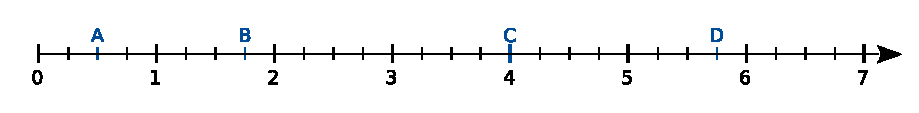
\includegraphics[width=15.5cm]{regle_ABCD07} \end{center}
\begin{enumerate}
 \item Donne de deux façons différentes les abscisses des points $A$, $B$, $C$ et $D$ ;
 \item Donne de deux façons différentes l'abscisse du point situé exactement au milieu des points $A$ et $B$ puis celui du point situé exactement au milieu de $C$ et $D$.
 \end{enumerate}
\end{partie}

\begin{partie}
Dessine une demi‑droite graduée et partage l'unité en 12 parts égales :
\begin{enumerate}
 \item Combien de ces parts faut‑il prendre pour avoir $\dfrac{1}{6}$ de l'unité ? Même question pour $\dfrac{1}{3}$, $\dfrac{1}{4}$ puis $\dfrac{1}{2}$ ;
 \item Place sur cette demi‑droite les points $E$, $F$, $G$ et $H$ d'abscisses respectives $\dfrac{13}{12}$, $\dfrac{2}{3}$, $\dfrac{3}{2}$ et $\dfrac{5}{4}$ ;
 \item Donne de deux façons différentes l'abscisse du point $K$ situé exactement au milieu de $G$ et $H$.
 \end{enumerate}
\end{partie}

\end{activite}

%%%%%%%%%%%%%%%%%%%%%%%%%%%%%%%%%%%%%%%%%%%%%%%%%%%%%%%%%%%%%%%%%%%%%%%%

\begin{activite}[Égalités de fractions]

\begin{partie}[De l'observation et de l'imagination \ldots]
On a représenté ci‑dessous trois fois le même rectangle avec la même surface coloriée. Chacun d'entre eux a été partagé en parts égales de différentes façons : \\[0.5em]
\begin{minipage}[c]{0.32\linewidth}
 
\includegraphics[width=3.2cm]{surface_coloriee}
\end{minipage} \hfill%
\begin{minipage}[c]{0.32\linewidth}
 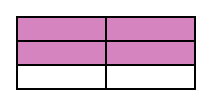
\includegraphics[width=3.2cm]{surface_coloriee2}
 \end{minipage} \hfill%
\begin{minipage}[c]{0.32\linewidth} 
 
\includegraphics[width=3.2cm]{surface_coloriee3}
 \end{minipage} \\
\begin{enumerate}
 \item Pour chacun d'entre eux, quelle fraction du rectangle est coloriée en rose ? \label{NbsRatio_acti3}
 \item À l'aide de la question \ref{NbsRatio_acti3}, complète l'égalité suivante : $\dfrac{2}{3} = \dfrac{\ldots \ldots}{\ldots \ldots} = \dfrac{\ldots \ldots}{\ldots \ldots}$.
 \item En utilisant une méthode similaire, écris trois fractions égales à $\dfrac{10}{12}$.
 \item Est-il possible de trouver une fraction égale à $\dfrac{7}{9}$ ayant pour dénominateur 81 ? Ayant pour dénominateur 11 ? 
 \end{enumerate}
\end{partie}

\begin{partie}[Avec des demi-droites graduées (d'après IREM de Bordeaux)]
Décalque l'ensemble des demi-droites graduées ci‑dessous : \\[0.5em]
\begin{center} 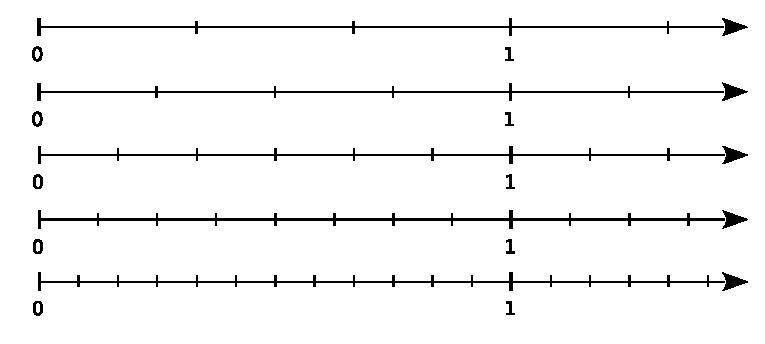
\includegraphics[width=13cm]{ddroites_graduees} \end{center}
\begin{enumerate}
 \item Choisis la demi‑droite graduée qui convient le mieux pour placer chacun des nombres suivants : $\dfrac{4}{3}$ ; $\dfrac{8}{6}$ et $\dfrac{16}{12}$. Que remarques‑tu ?
 \item Place $\dfrac{3}{4}$ sur la demi-droite graduée appropriée et déduis-en des fractions égales à $\dfrac{3}{4}$.
 \item En t'inspirant de ce qui précède, propose des fractions égales à 2 puis à 5.
 \end{enumerate}
\end{partie}

\begin{partie}[Avec la définition du quotient]
\begin{enumerate}
 \item Calcule les produits suivants :
 \begin{colitemize}{6}
  \item $2 \cdot 1,5$ ;
  \item $ 6 \cdot 1,5$ ; 
  \item $8 \cdot 1,5$ ;
  \item $10 \cdot 1,5$ ; 
  \item $12 \cdot 1,5$ ; 
  \item $22 \cdot 1,5$.
 \end{colitemize}
 \item À l'aide de la définition du quotient, déduis‑en des fractions égales à 1,5.
 \end{enumerate}
\end{partie}

\begin{partie}[Synthèse]
À l'aide de ce qui précède, détermine la condition pour que deux fractions soient égales.
\end{partie}

\begin{partie}[Des applications]
\begin{enumerate}
 \item Trouve une fraction « plus simple » (c'est-à-dire avec un \textbf{numérateur} et un \textbf{dénominateur} plus petits) égale à $\dfrac{35}{14}$ ;
 \item En détaillant ta démarche, détermine une fraction égale à $\dfrac{5,1}{0,75}$.
 
Simplifie, si possible, cette fraction.
 \end{enumerate}
\end{partie}

\end{activite}

%%%%%%%%%%%%%%%%%%%%%%%%%%%%%%%%%%%%%%%%%%%%%%%%%%%%%%%%%%%%%%%%%%%%%%%%

\begin{activite}[Comparaisons dans les cas simples]

\begin{center} 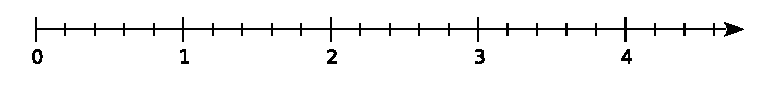
\includegraphics[width=12.6cm]{regle01234_bis} \end{center}

Lola la tortue et Jeannot le lapin décident de faire une course sur la demi-droite graduée ci-dessus. Le point de départ est l'origine de la demi-droite. Lola parcourt $\dfrac{7}{5}$ d'unité et Jeannot parcourt $\dfrac{12}{5}$ d'unité.

\begin{enumerate}
 \item Reproduis la demi-droite graduée ci-dessus puis places-y les points $L$ et $J$ pour indiquer les positions de Lola et de Jeannot. 
 \item Lequel des deux a parcouru le plus grand trajet ? Parmi les fractions $\dfrac{7}{5}$ et $\dfrac{12}{5}$, quelle est la plus grande ? \label{NbsRatio_acti4}
 \item En t'aidant de la question \ref{NbsRatio_acti4}, énonce une règle qui permet de comparer des fractions de même dénominateur. 
 \item Applique la règle que tu as trouvée pour comparer $\dfrac{25}{109}$ et $\dfrac{38}{109}$ puis $\dfrac{7,9}{23}$ et $\dfrac{7,09}{23}$.
\end{enumerate}

\end{activite}

%%%%%%%%%%%%%%%%%%%%%%%%%%%%%%%%%%%%%%%%%%%%%%%%%%%%%%%%%%%%%%%%%%%%%%%%

\begin{activite}[Comparaisons dans les cas complexes]

\begin{center} 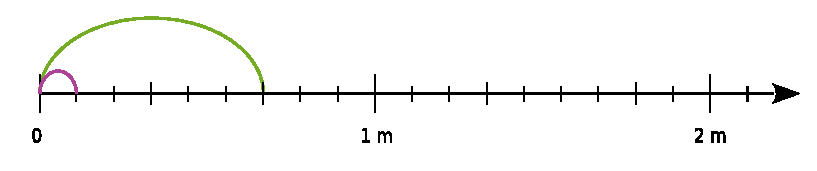
\includegraphics[width=13.5cm]{regle_kangourou} \end{center}

Zouzou le kangourou et Charlotte la puce décident de faire une course sur la demi-droite graduée ci-dessus. Le point de départ est l'origine de la demi-droite. Zouzou fait des bonds de $\dfrac{2}{3}$ de mètre (en vert) tandis que Charlotte fait des bonds de $\dfrac{1}{9}$ de mètre (en rose).

\begin{enumerate}
 \item Charlotte a fait 11 bonds tandis que Zouzou n'en a fait que 2. Reproduis la demi-droite graduée ci-dessus puis places-y les points $C$ et $Z$ pour indiquer les positions de Charlotte et de Zouzou. 
 \item Complète les phrases suivantes : \label{NbsRatio_acti5}
 \begin{itemize}
  \item « Charlotte a parcouru $\dfrac{\ldots \ldots}{9}$ de mètre. »
  \vspace{0.2cm}
  \item « Zouzou a parcouru $\dfrac{\ldots \ldots}{3}$ de mètre, ce qui équivaut à $\dfrac{\ldots \ldots}{9}$ de mètre. »
  \end{itemize}
  \vspace{0.2cm}
 \item En t'aidant de la question \ref{NbsRatio_acti5}, indique lequel des deux a parcouru le plus grand trajet. Parmi les fractions $\dfrac{11}{9}$ et $\dfrac{4}{3}$, quelle est la plus grande ? 
 \item Énonce une règle qui permet de comparer des fractions de dénominateurs différents.
 \item Applique la règle que tu as trouvée pour comparer $\dfrac{8}{3}$ et $\dfrac{39}{15}$ puis $\dfrac{2,1}{12}$ et $\dfrac{6,03}{36}$.
 \end{enumerate}

\end{activite}

%%%%%%%%%%%%%%%%%%%%%%%%%%%%%%%%%%%%%%%%%%%%%%%%%%%%%%%%%%%%%%%%%%%%%%%%

\begin{activite}[Prendre une fraction d'une quantité]

\begin{minipage}[c]{0.7\linewidth}
\begin{partie}[C'est pas de la tarte !]
\begin{enumerate}
 \item Florence a acheté une tarte de 400 g qu'elle a partagée en huit parts égales. Très gourmande, elle en a mangé les trois huitièmes. Calcule la masse d'une part de tarte et déduis-en la quantité, en grammes, mangée par Florence.
 \item Pour fêter son anniversaire, Patrice a acheté trois tartes identiques à celle de Florence.
 
À la fin de la fête, il annonce fièrement : « J'ai mangé le huitième des tartes ! ». Quelle quantité de tarte, en grammes, a‑t‑il mangée ?
 \item Quelle autre opération permet de retrouver les réponses précédentes ?
 
Complète alors : « Prendre les $\dfrac{3}{8}$ de 400 revient à \ldots . ».
 \end{enumerate}
\end{partie}
\end{minipage} \hfill%
\begin{minipage}[c]{0.27\linewidth}
\begin{center} 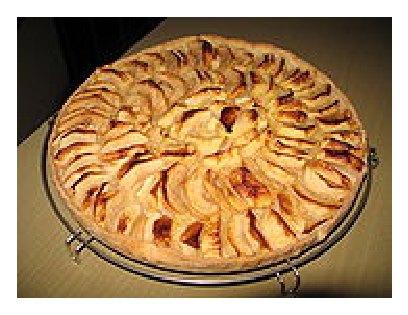
\includegraphics[width=4cm]{tarte_pommes} \end{center}
\begin{center} \quad \small{Copyleft Manuel Flury \newline \phantom{...} Wikimedia commons \newline \phantom{..} Licence GNU-FDL 1.2} \end{center}
\end{minipage} \\

\begin{partie}[Histoire de sous \ldots]
Mario devait 5 sésames (monnaie utilisée en Sésamathie, pays des sésamatheux) à Bastien. 
Comme il ne les a pas rendus en temps et en heure, Bastien lui réclame des intérêts en lui demandant maintenant de lui donner les sept tiers de cette somme.
\begin{enumerate}
 \item Mario se dit que « prendre 7 tiers de 5, c'est prendre 7 fois le tiers de 5. Or le tiers de 5, c'est le quotient de 5 par 3, soit exactement \ldots ». \\[0.5em]
Poursuis son raisonnement pour déterminer la somme exacte à rembourser.
 \item Complète : « Prendre les $\dfrac{7}{3}$ de 5 revient à \ldots . ».
 \end{enumerate}
\end{partie}

\end{activite}

%%%%%%%%%%%%%%%%%%%%%%%%%%%%%%%%%%%%%%%%%%%%%%%%%%%%%%%%%%%%%%%%%%%%%%%%

\begin{activite}[Quelques applications]

\begin{partie}[Question de méthode !]
\begin{enumerate}
 \item Calcule chacun des produits suivants de trois façons différentes :
 \begin{colitemize}{3}
  \item $8 \cdot \dfrac{7}{4}$ ;
  \item $2,5 \cdot \dfrac{2}{5}$ ; 
  \item $ \dfrac{12}{6} \cdot 9$.
   \end{colitemize}
   \vspace{0.3cm}
Dans chaque cas, y a‑t‑il une méthode plus simple que les autres ? Explique.
 \item Pour trouver une écriture décimale exacte de $21 \cdot \dfrac{3}{7}$, Chloé affirme qu'on ne peut pas utiliser l'une des méthodes. A‑t‑elle raison ? Explique.
 \item Choisis la méthode qui te semble la plus astucieuse pour calculer les produits suivants :
 \begin{colitemize}{3}
  \item $1,89 \cdot \dfrac{100}{9}$ ;
  \item $15 \cdot \dfrac{2}{3}$ ; 
  \item $45 \cdot \dfrac{8}{4}$.
   \end{colitemize}
 \item On voudrait trouver la valeur exacte de $5 \cdot \dfrac{7}{3}$. Calcule ce produit en utilisant les trois méthodes. Quelle réponse donnerais‑tu à la question posée ?
 \end{enumerate}
\end{partie}

\begin{partie}[Multiplier par 0,1 ; par 0,01 ; \ldots]
\begin{enumerate}
 \item En remplaçant 0,1 par une fraction décimale, calcule $5,4 \cdot 0,1$.
 
De la même façon, calcule $0,791 \cdot 0,001$ puis $2\,009 \cdot 0,01$.
 \item Quelle autre opération peut‑on effectuer à la place d'une multiplication par 0,1 ? Par 0,01 ? Et par 0,001 ?
 \end{enumerate}
\end{partie}

\begin{partie}[Des conversions]
\begin{enumerate}
 \item Complète : $56,5 \text{cm} = 56,5 \cdot \ldots \text{cm} = 56,5 \cdot \dfrac{1}{\ldots} \text{m} = \bigg(56,5 \cdot \dfrac{1}{\ldots} \bigg) \text{m} =\dfrac{\ldots}{\ldots} \, \text{m} = \ldots \text{m}$.
 \item En reproduisant un raisonnement du même type, convertis 87,2 mm en m.
 \end{enumerate}
\end{partie}

\end{activite}

%%%%%%%%%%%%%%%%%%%%%%%%%%%%%%%%%%%%%%%%%%%%%%%%%%%%%%%%%%%%%%%%%%%%%%%%

\begin{activite}[Appliquer un taux de pourcentage]

\begin{partie}
Un commerçant consent une remise de 18 \% sur tous ses articles :
\begin{enumerate}
 \item Combien représente cette remise sur un article valant 100 CHF au départ ?
 
Même question pour un article valant 1 CHF, puis pour un article valant 135 CHF au départ.
 \item Par quel nombre faut-il multiplier le prix de départ d'un article (en CHF) pour connaître le montant de la remise (en CHF) ? (Tu donneras ce nombre sous la forme d'une fraction décimale).
 \item Complète : « Prendre 18 \% d'un nombre revient à \ldots . ».
 \end{enumerate}
\end{partie}

\begin{partie}
Dans un magasin, un article coûte 240 CHF. Calcule le montant de la remise lorsque celle‑ci est de 50 \%. Que remarques‑tu ? À quelle fraction du prix de cet article correspond cette remise ? Mêmes questions pour une remise de 25 \% puis de 75 \%.
\end{partie}

\begin{partie}
Dans un autre magasin, on accorde 16 \% de remise sur un article coûtant 300 CHF.

Détermine astucieusement le montant de cette remise.
\end{partie}

\end{activite}

%%%%%%%%%%%%%%%%%%%%%%%%%%%%%%%%%%%%%%%%%%%%%%%%%%%%%%%%%%%%%%%%%%%%%%%%

\begin{activite}[Additions et soustractions]

\begin{enumerate}
 \item Complète par des fractions les phrases suivantes :
 
 \begin{minipage}[c]{0.68\linewidth}
 \begin{itemize}
  \item L'aire de la région verte représente $\dfrac{3}{\ldots}$ de l'aire totale ;
  \vspace{0.3cm}
  \item L'aire de la région rose représente $\dfrac{1}{\ldots}$ de l'aire totale.
  \end{itemize}
  \end{minipage} \hfill%
  \begin{minipage}[c]{0.28\linewidth}
  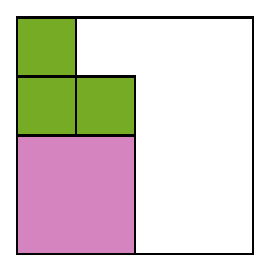
\includegraphics[width=3.6cm]{regions_vertesroses}
   \end{minipage} \\
 \item Écris le calcul à effectuer pour obtenir l'aire que représente la région coloriée par rapport à l'aire totale.
 \item Reproduis le carré ci-contre puis effectue des tracés judicieux pour obtenir ce que représente l'aire des deux régions verte et rose par rapport à l'aire totale. 
 \item Complète l'égalité suivante : $\dfrac{3}{16} + \dfrac{1}{4} = \dfrac{\ldots \ldots}{\ldots \ldots}$.
 \vspace{0.2cm}
 \item Que faudrait-il faire pour retrouver ce résultat par le calcul ?
 \item Énonce une règle qui permet d'additionner ou de soustraire des fractions de dénominateurs différents. 
 \item Applique la règle que tu as trouvée pour effectuer le calcul suivant : $\dfrac{2}{5} + \dfrac{1}{30}$.
\end{enumerate}

\end{activite}

%%%%%%%%%%%%%%%%%%%%%%%%%%%%%%%%%%%%%%%%%%%%%%%%%%%%%%%%%%%%%%%%%%%%%%%%


\cours
%\section{Une section}

% remarque : pour qu'un mot se retrouve dans le lexique : \MotDefinition{asymptote horizontale}{} 

\begin{aconnaitre}
La \MotDefinition{fraction}{} $\dfrac{a}{\textcolor{C1}{b}}$ est le quotient de l'entier relatif $a$ par l'entier relatif $\textcolor{C1}{b}$ (avec $\textcolor{C1}{b} \neq 0$), ainsi :

$\dfrac{a}{\textcolor{C1}{b}} = a : \textcolor{C1}{b}$. Le nombre $a$ s'appelle le \MotDefinition{numérateur}{}, $\textcolor{C1}{b}$ est le \MotDefinition{dénominateur}{} et le trait horizontal est la \MotDefinition{barre de fraction}{}. Un nombre \MotDefinition{rationnel}{} est un nombre qui peut s'écrire comme une fraction.
\end{aconnaitre}


\begin{methode*1}[Utiliser la définition du quotient]

\begin{exemple*1}
Parmi les nombres suivants : $\dfrac{3}{4}$, $\dfrac{23}{2,3}$, $\dfrac{13}{15}$, $\dfrac{0}{10}$, $\dfrac{1,2}{5}$, détermine ceux qui ne sont pas une fraction.

Une fraction possède un numérateur \textbf{et} un dénominateur entier. Donc $\dfrac{23}{2,3}$ et $\dfrac{1,2}{5}$ ne sont pas des fractions.
 \end{exemple*1}
 
\begin{remarque}
Les quotients $\dfrac{23}{2,3}$, $\dfrac{1,2}{5}$ utilisent l'écriture fractionnaire mais ne sont pas des fractions. Par contre ce sont des nombres rationnels car $\dfrac{23}{2,3} = 10$ et $\dfrac{1,2}{5} = 0,24$.
 \end{remarque}
 
  \exercice  
%\correction

 \end{methode*1}

%%%%%%%%%%%%%%%%%%%%%%%%%%%%%%%%%%%%%%%%%%%%%%%%%%%%%%%%%%%%%%%%%%

\begin{aconnaitre}
Une \MotDefinition{fraction décimale}{} est une fraction dont le dénominateur est 1, 10, 100, 1\,000 \ldots
Un nombre pouvant s'écrire sous la forme d'une fraction décimale est un \MotDefinition{nombre décimal}{}. Il peut aussi se noter en utilisant une virgule ; c'est son \MotDefinition{écriture décimale}{}.
\end{aconnaitre}

\begin{methode*1}

\begin{exemple*1}
Donne l'écriture décimale du nombre $\dfrac{567}{10}$ :\\[0.5em]
L'écriture décimale est obtenue en calculant la division $567 : 10 = 56,7$.
 \end{exemple*1}
 
\begin{exemple*1}
Écris 0,25 sous la forme d'une fraction décimale. \\[0.5em]
Une fraction décimale a pour dénominateur 1, 10, 100, 1\,000, \ldots .

Le chiffre 5 occupe la position des centièmes.

On obtient la fraction décimale $0,25 = \dfrac{25}{100}$.
 \end{exemple*1}
 
  \exercice
Donne l'écriture décimale des nombres :
\begin{colenumerate}{3}
 \item $\dfrac{12}{5}$ ;
 \item $\dfrac{2,5}{2}$ ;
 \item $\dfrac{4}{2,5}$.
 \end{colenumerate}
%\correction

  \exercice
Écris les nombres suivants sous la forme d'une fraction décimale :
\begin{colenumerate}{3}
 \item $0,8$ ;
 \item $0,12$ ;
 \item $1,541$.
 \end{colenumerate}
%\correction

 \end{methode*1}

%%%%%%%%%%%%%%%%%%%%%%%%%%%%%%%%%%%%%%%%%%%%%%%%%%%%%%%%%%%%%%%%%%

\begin{methode*1}[Fraction d'un tout]

\begin{exemple*1}
\begin{minipage}[c]{0.4\linewidth}
Détermine quelle fraction de la figure est colorée.
 \end{minipage} \hfill%
 \begin{minipage}[c]{0.4\linewidth}
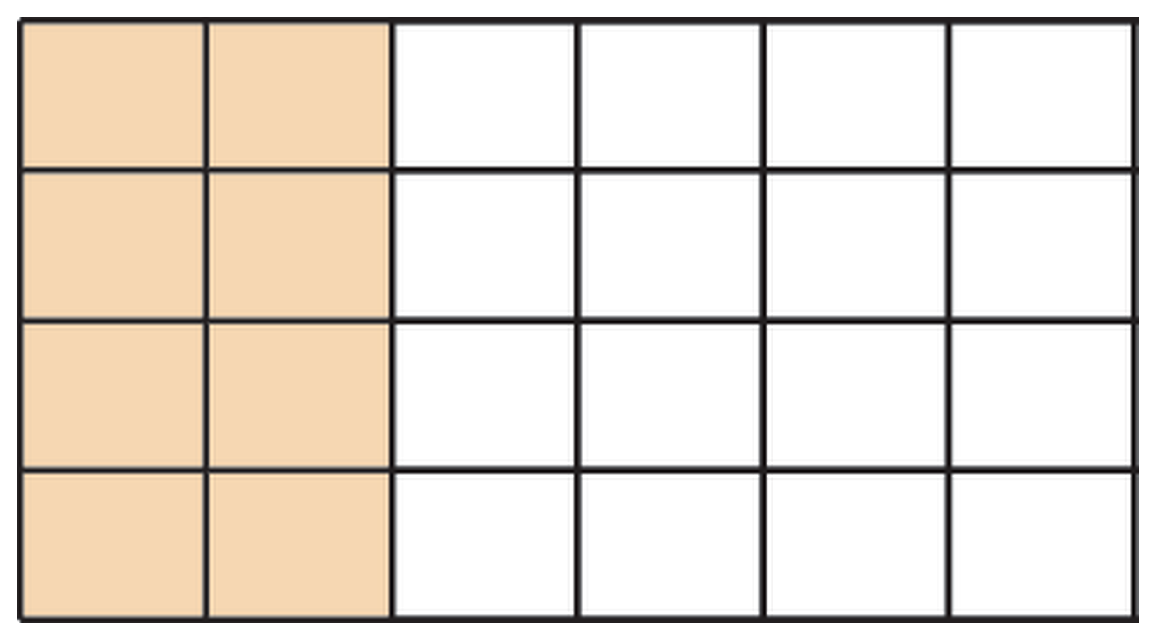
\includegraphics[width=3cm]{fraction_figure}
 \end{minipage} \\[1em]
La figure est divisée en 24 parties identiques et 8 sont colorées. On a coloré les $\dfrac{8}{24}$ de la figure.
 \end{exemple*1}
 
\begin{remarque}
La division de la figure aurait pu être en 12 parties identiques dont 4 sont colorées, c'est-à-dire, $\dfrac{4}{12}$ de la figure ou les $\dfrac{2}{6}$ de la figure ou les $\dfrac{1}{3}$ de la figure. Mais toutes ces fractions sont égales.
 \end{remarque}

  \exercice
Pour chaque figure donne la fraction de la partie colorée :
\begin{colenumerate}{3}
 \item 
 
 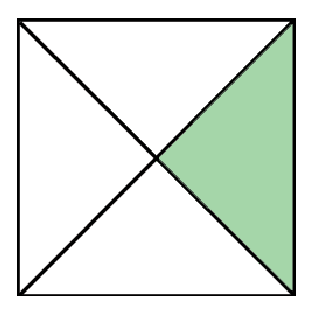
\includegraphics[width=1.7cm]{fraction_verte}
 \item 
 
 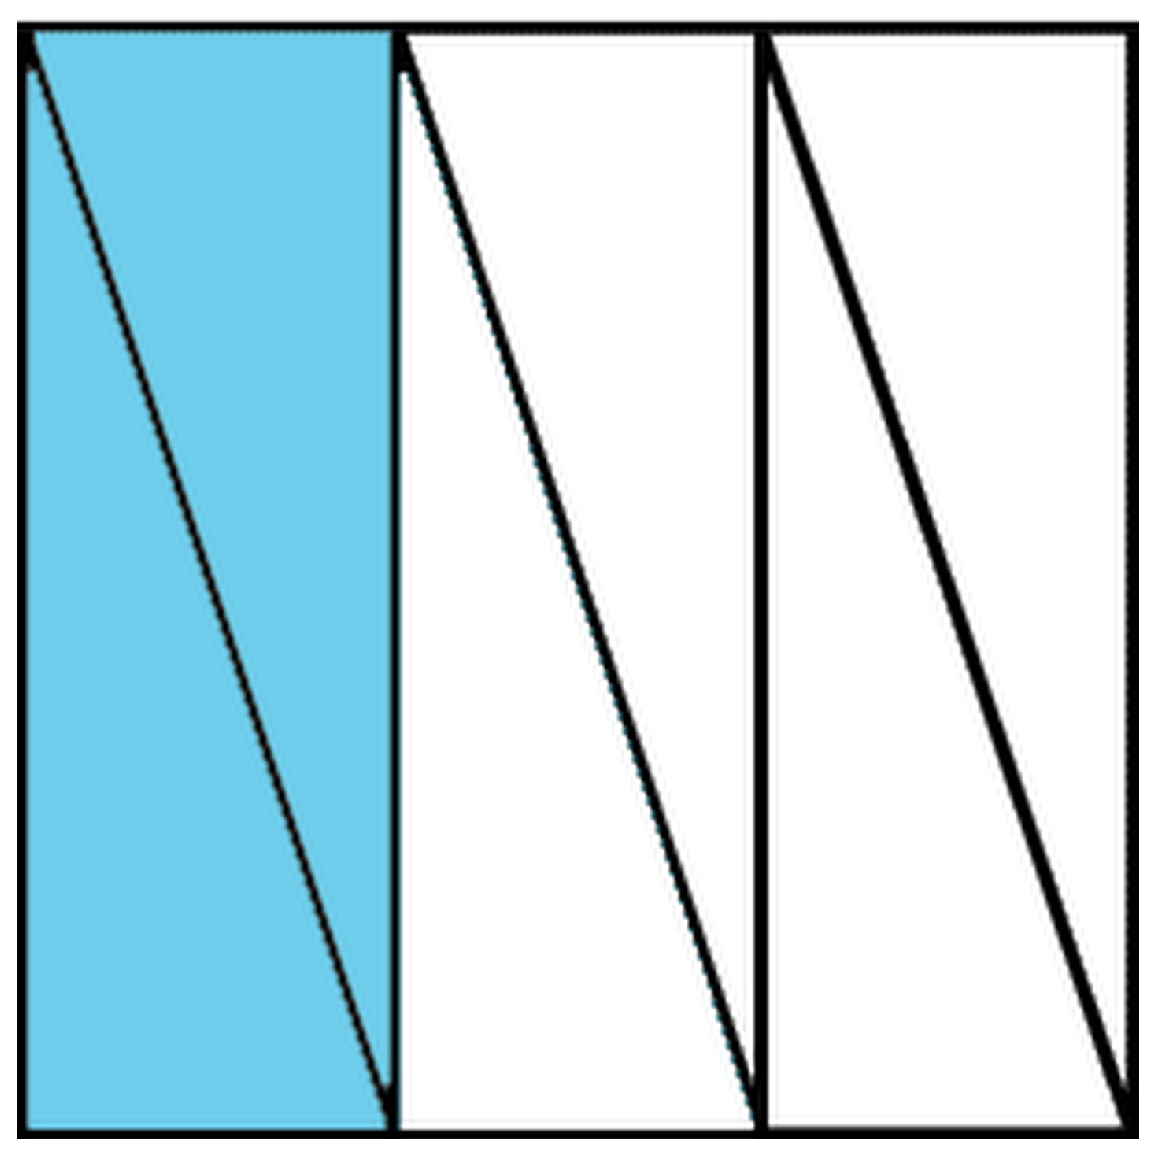
\includegraphics[width=1.7cm]{fraction_bleu}
 \item 
 
 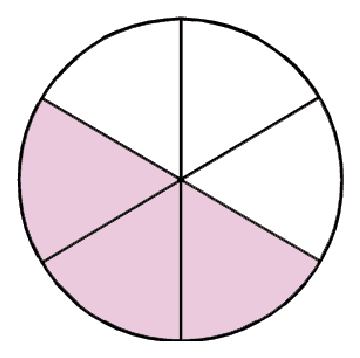
\includegraphics[width=1.7cm]{fraction_rose}
 \end{colenumerate}  
%\correction

 \end{methode*1}

%%%%%%%%%%%%%%%%%%%%%%%%%%%%%%%%%%%%%%%%%%%%%%%%%%%%%%%%%%%%%%%%%%

\begin{methode*1}[Placer le quotient de deux entiers sur une demi‑droite graduée]

\begin{exemple*1}
Place sur une même demi‑droite graduée les points $A$ et $B$ d'abscisses respectives $\dfrac{5}{6}$ et $\dfrac{11}{3}$. \\[1em]
On choisit une longueur unité $OI$ que l'on partage en six parts égales. Chacune de ces parts correspond donc à \textcolor{C1}{$\dfrac{1}{6}$} de l'unité.
\begin{itemize}
 \item Pour placer le point $A$, on utilise $\dfrac{5}{6} = 5 \cdot \dfrac{1}{6}$ et on reporte donc cinq \textcolor{C1}{sixièmes} à partir du point $O$.
 \begin{center} 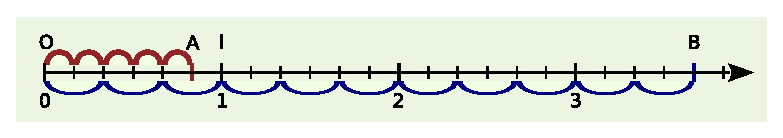
\includegraphics[width=10cm]{quotient_ddroite} \end{center}
 \item Pour placer le point $B$, on remarque que deux parts correspondent à $\dfrac{1}{3}$ de l'unité et on utilise $\dfrac{11}{3} = 11 \cdot \dfrac{1}{3}$. On reporte donc 11 tiers à partir du point $O$.
 \end{itemize}
 \end{exemple*1}
 
 
 \exercice
 Sur une même demi‑droite graduée, place les points $E \bigg(\dfrac{3}{4} \bigg)$ ; $F \bigg(2 - \dfrac{1}{4} \bigg)$ et $G \bigg(\dfrac{5}{2} \bigg)$.
%\correction

 \end{methode*1}

%%%%%%%%%%%%%%%%%%%%%%%%%%%%%%%%%%%%%%%%%%%%%%%%%%%%%%%%%%%%%%%%%%

\begin{aconnaitre}
Un quotient ne change pas quand on \textbf{multiplie} ou qu'on \textbf{\textcolor{A1}{divise}} son numérateur et son dénominateur par un \textbf{même nombre} non nul :
\begin{center} $\dfrac{a}{b} = \dfrac{a \cdot \textcolor{C1}{k}}{b \cdot \textcolor{C1}{k}}$ ou $\dfrac{a}{b} = \dfrac{a : \textcolor{C1}{k}}{b : \textcolor{C1}{k}}$ où $a$, $b$ et $k$ sont des nombres, avec $b \neq 0$ et $k \neq 0$. \end{center}
\end{aconnaitre}


\begin{methode*1}[Reconnaître des écritures fractionnaires égales]

\begin{exemple*1}
Montre que $\dfrac{5}{7}$ et $\dfrac{40}{56}$ représentent un même nombre. \\[1em]
On sait que $5 \cdot \text{\textbf{\textcolor{C2}{8}}} = 40$ et que $7 \cdot \text{\textbf{\textcolor{C2}{8}}} = 56$. 
En multipliant le numérateur et le dénominateur par le même nombre, on obtient $\dfrac{5}{7} = \dfrac{5 \cdot \text{\textbf{\textcolor{C2}{8}}}}{7 \cdot \text{\textbf{\textcolor{C2}{8}}}} = \dfrac{40}{56}$, ce qui signifie que $\dfrac{5}{7}$ et $\dfrac{40}{56}$ représentent le même nombre.
 \end{exemple*1}
 
 \begin{exemple*1}
Parmi  $\dfrac{21}{27}$ ; $\dfrac{56}{81}$ ; $\dfrac{0,7}{0,9}$ ; $\dfrac{48}{63}$ et $\dfrac{23,1}{29,7}$ relève les nombres égaux à $\dfrac{7}{9}$. \\[1em]
\begin{itemize}
 \item $\dfrac{7}{9} = \dfrac{7 \cdot \text{\textbf{\textcolor{C2}{3}}}}{9 \cdot \text{\textbf{\textcolor{C2}{3}}}} = \dfrac{21}{27}$ donc $\dfrac{7}{9} = \dfrac{21}{27}$ ;
\vspace{0.3cm}
\item $\dfrac{0,7}{0,9} = \dfrac{0,7 \cdot \text{\textbf{\textcolor{C2}{10}}}}{0,9 \cdot \text{\textbf{\textcolor{C2}{10}}}} = \dfrac{7}{9}$ donc $\dfrac{7}{9} = \dfrac{0,7}{0,9}$ ;
  \item On remarque que $7 \cdot \text{\textbf{\textcolor{C2}{8}}} = 56$ et que $9 \cdot 8 = 72$ donc $\dfrac{7}{9} = \dfrac{7 \cdot \text{\textbf{\textcolor{C2}{8}}}}{9 \cdot \text{\textbf{\textcolor{C2}{8}}}} = \dfrac{56}{72}$ et $\dfrac{7}{9} \neq \dfrac{56}{81}$;
  \item On remarque que $9 \cdot \text{\textbf{\textcolor{C2}{7}}} = 63$ et que $7 \cdot 7 = 49$ donc $\dfrac{7}{9} = \dfrac{7 \cdot \text{\textbf{\textcolor{C2}{7}}}}{9 \cdot \text{\textbf{\textcolor{C2}{7}}}} = \dfrac{49}{63}$ et $\dfrac{7}{9} \neq \dfrac{48}{63}$ ; 
 \vspace{0.3cm}
  \item On détermine le nombre qui multiplié par 7 donne 23,1. Ce nombre est $\dfrac{23,1}{7}$. En effectuant la division, on trouve $23,1 : 7 = 3,3$.

Or $9 \cdot 3,3 = 29,7$ donc $\dfrac{7}{9} = \dfrac{7 \cdot \text{\textbf{\textcolor{C2}{3,3}}}}{9 \cdot \text{\textbf{\textcolor{C2}{3,3}}}} = \dfrac{23,1}{29,7}$.
 \end{itemize}
Les écritures fractionnaires de la liste égales à $\dfrac{7}{9}$ sont donc $\dfrac{21}{27}$ ; $\dfrac{0,7}{0,9}$ ; $\dfrac{23,1}{29,7}$.
 \end{exemple*1}
 
 
  \exercice
Parmi les nombres $\dfrac{45}{27}$ ; $\dfrac{0,05}{0,03}$ ; $\dfrac{54}{33}$ ; $\dfrac{90}{54}$ et $\dfrac{40}{25}$ relève ceux qui sont

égaux à $\dfrac{5}{3}$.
%\correction

  \exercice
  Trouve une fraction égale à chaque fraction de la liste $\dfrac{40}{90}$ ; $\dfrac{18}{72}$ ; $\dfrac{16}{24}$ et $\dfrac{125}{75}$.
%\correction

 \end{methode*1}

%%%%%%%%%%%%%%%%%%%%%%%%%%%%%%%%%%%%%%%%%%%%%%%%%%%%%%%%%%%%%%%%%%

\begin{aconnaitre}
\MotDefinition{Amplifier une fraction}{} consiste à obtenir une fraction égale en multipliant le numérateur et le dénominateur par le même nombre entier non nul. \\[0.5em]
\MotDefinition{Simplifier ou réduire une fraction}{} consiste à obtenir une fraction égale en divisant le numérateur et le dénominateur par le même nombre entier non nul. \\[0.5em]
Une \MotDefinition{fraction irréductible}{} est une fraction qu'on ne peut plus simplifier.
\end{aconnaitre}


\begin{methode*1}[Simplifier une fraction]

\begin{exemple*1}
Rends la fraction $\dfrac{48}{60}$ irréductible. \\[1em]
On utilise les critères de divisibilité connus et les tables de multiplication :
\begin{itemize}
 \item Le chiffre des unités de 48 est 8 et celui de 60 est 0 donc 48 et 60 sont divisibles par 2. 
Ainsi $\dfrac{48}{60} = \dfrac{\text{\textbf{\textcolor{C2}{2}}} \cdot 24}{\text{\textbf{\textcolor{C2}{2}}} \cdot 30} = \dfrac{24}{30}$ On dit qu'on a \textbf{simplifié} la fraction $\dfrac{48}{60}$ par 2.
 \item On remarque que 24 et 30 sont des multiples de 6. On peut donc encore simplifier la fraction par 6.
 Ainsi $\dfrac{24}{30} = \dfrac{\text{\textbf{\textcolor{C2}{6}}} \cdot 4}{\text{\textbf{\textcolor{C2}{6}}} \cdot 5} = \dfrac{4}{5}$.
 \end{itemize}
Une fraction plus simple égale à $\dfrac{48}{60}$ est donc par exemple $\dfrac{24}{30}$ ou encore $\dfrac{4}{5}$.
$\dfrac{4}{5}$ n'est plus simplifiable. C'est la fraction irréductible égale à $\dfrac{48}{60}$.
 \end{exemple*1}
 
\begin{exemple*1}
Écris 2,5 sous la forme d'une fraction irréductible : \\[1em]
$2,5 = \dfrac{25}{10} = \dfrac{5 \cdot \text{\textbf{\textcolor{C2}{5}}}}{2 \cdot \text{\textbf{\textcolor{C2}{5}}}} = \dfrac{5}{2}$.
 \end{exemple*1}
 
 
  \exercice
Rends irréductible les fractions : $\dfrac{27}{36}$, $\dfrac{75}{30}$, $\dfrac{45}{39}$.
%\correction

  \exercice
Simplifie $\dfrac{20}{12}$ puis trouve un autre quotient égal dont le dénominateur est 21.
%\correction

  \exercice
Écris les nombres suivants sous la forme d'une fraction irréductible :
\begin{colenumerate}{3}
 \item 0,5 ;
 \item 1,5 ;
 \item 0,8.
 \end{colenumerate}
%\correction

 \end{methode*1}

%%%%%%%%%%%%%%%%%%%%%%%%%%%%%%%%%%%%%%%%%%%%%%%%%%%%%%%%%%%%%%%%%%

\begin{aconnaitre}
Pour \MotDefinition{comparer des nombres en écriture fractionnaire}{}, on les écrit avec le même dénominateur, puis on les range dans le même ordre que leurs numérateurs. \\[0.5em]
Si le numérateur d'un nombre en écriture fractionnaire est supérieur à son dénominateur, alors il est supérieur à 1. Si son numérateur est inférieur à son dénominateur alors il est inférieur à 1.
\end{aconnaitre}


\begin{methode*1}[Comparer]

\begin{exemple*1}
Compare les fractions $\dfrac{12}{4}$ et $\dfrac{57}{20}$ :
\begin{center}
 \begin{tabularx}{\linewidth}{ccX}
  $\dfrac{12}{4} = \dfrac{12 \cdot \text{\textbf{\textcolor{C2}{5}}}}{4 \cdot \text{\textbf{\textcolor{C2}{5}}}} = \dfrac{60}{20}$ & $\rightarrow$ & On écrit la fraction $\dfrac{12}{4}$ avec le dénominateur 20 ; \\
  $60 > 57$ & $\rightarrow$ & On compare les numérateurs ; \\[0.5em]
  d'où $\dfrac{60}{20} > \dfrac{57}{20}$ & $\rightarrow$ & On range les expressions fractionnaires dans le même ordre que leurs numérateurs ; \\ 
  $\dfrac{12}{4} > \dfrac{57}{20}$ & $\rightarrow$ & On conclut. \\
  \end{tabularx}
\end{center}
 \end{exemple*1}
 
  \exercice
Range dans l'ordre croissant les nombres : $\dfrac{21}{18}$; $\dfrac{5}{3}$ ; $\dfrac{10}{9}$.
%\correction

  \exercice
Range dans l'ordre décroissant les nombres : $\dfrac{6}{13}$ ; $\dfrac{9}{7}$ ; $\dfrac{2}{13}$ ; $\dfrac{11}{13}$ ; $\dfrac{17}{7}$.
%\correction

 \end{methode*1}

%%%%%%%%%%%%%%%%%%%%%%%%%%%%%%%%%%%%%%%%%%%%%%%%%%%%%%%%%%%%%%%%%%

\begin{aconnaitre}
Pour multiplier un nombre décimal \textcolor{B2}{$a$} par une fraction $\dfrac{\textcolor{PartieGeometrie}{b}}{\textcolor{H1}{c}}$ (avec $c \neq 0$),
\begin{itemize}
 \item on calcule le quotient $\textcolor{PartieGeometrie}{b} : \textcolor{H1}{c}$ puis on multiplie le résultat par \textcolor{B2}{$a$} ;
 \item ou on calcule le produit $\textcolor{B2}{a} \cdot \textcolor{PartieGeometrie}{b}$ puis on divise le résultat par \textcolor{H1}{$c$} ;
 \item ou on calcule le quotient $\textcolor{B2}{a} : \textcolor{H1}{c}$ puis on multiplie le résultat par \textcolor{PartieGeometrie}{$b$}.
 \end{itemize}
\end{aconnaitre}

\begin{aconnaitre}
\MotDefinition{Prendre une fraction d'une quantité}{}, c'est multiplier la fraction par la quantité.
\end{aconnaitre}


\begin{methode*1}[Prendre une fraction d'une quantité]

\begin{remarque}
Peu importe la méthode, on divise toujours par le dénominateur de la fraction.
 \end{remarque}

\begin{exemple*1}
Calcule $45 \cdot \dfrac{4}{5}$: \\[1em]
\begin{itemize}
 \item $45 \cdot \dfrac{4}{5} = 45 \cdot (4 : 5) = 45 \cdot 0,8 = 36$ ;
 \item ou $45 \cdot \dfrac{4}{5} = \dfrac{45 \cdot 4}{5} = \dfrac{180}{5} = 36$ ;
 \item ou $45 \cdot \dfrac{4}{5} = \dfrac{45}{5} \cdot 4 = 9 \cdot 4 = 36$.
 \end{itemize}
 \end{exemple*1}

\begin{remarque}
La dernière méthode semble ici plus rapide car les calculs peuvent se faire aisément de tête.
 \end{remarque}
 
 
\begin{exemple*1}
Amélie a dépensé les cinq septièmes de ses économies qui s'élevaient à 14,70 CHF. Calcule le montant de sa dépense. \\[1em]
Calculer les cinq septièmes de 14,7, c'est multiplier $\dfrac{5}{7}$ par 14,7. \\[0.5em]
$\dfrac{5}{7} \cdot 14,7 = \dfrac{14,7}{7} \cdot 5 = 2,1 \cdot 5 = 10,5$. (C'est ici la méthode la plus simple).\\[0.5em]
Amélie a donc dépensé 10,50 CHF.
 \end{exemple*1}
 
 
\begin{exemple*1}
36 \% des 425 élèves d'un collège sont externes. Combien d'élèves de ce collège sont externes ? \\[1em]
Prendre 36 \% de 425, c'est multiplier $\dfrac{36}{100}$ par 425.\\[0.5em]
$\dfrac{36}{100} \cdot 425 = \dfrac{36 \cdot 425}{100} = \dfrac{15\,300}{100} = 153$ \\[0.5em]
Il y a donc 153 élèves externes dans ce collège.
 \end{exemple*1}
 
  \exercice
Calcule :
\begin{colenumerate}{3}
 \item $5,6 \cdot \dfrac{10}{7}$ ;
 \item $45 \cdot \dfrac{9}{5}$ ;
 \item $4,6 \cdot \dfrac{18}{9}$ ; 
 \end{colenumerate}
%\correction

  \exercice
Les deux tiers des 60 salariés d'une entreprise sont des ouvriers, un quart sont des techniciens et les autres sont des cadres. Détermine le nombre de salariés dans chacune des catégories.
%\correction

  \exercice
Lundi, sur 23 kg de raisin récoltés, le vigneron a dû en jeter 12 \%. Quelle masse de raisin a‑t‑il jetée lundi ?
%\correction

 \end{methode*1}

%%%%%%%%%%%%%%%%%%%%%%%%%%%%%%%%%%%%%%%%%%%%%%%%%%%%%%%%%%%%%%%%%%


\begin{aconnaitre}
Pour \MotDefinition{additionner ou soustraire des fractions}{} :
\begin{itemize}
 \item on met les fractions au même dénominateur, en amplifiant ou en simplifiant ; 
 \item on additionne ou on soustrait les numérateurs et on garde le dénominateur commun.
 \end{itemize}
\end{aconnaitre}


\begin{methode*1}[Additionner ou soustraire des fractions]

\begin{exemple*1}
Calcule l'expression $A = \dfrac{7}{3} + \dfrac{5}{4}$ : \\[1em]
\begin{center}
 \begin{tabularx}{1.05\linewidth}{ccX}
  \phantom{.....}Multiples de 3 :  3 ; 6 ; 9 ; \fcolorbox{B2}{A4}{12} ; 15 ; \ldots & & \\
  Multiples de 4 : 4 ; 8 ; \fcolorbox{B2}{A4}{12} ; 16 ; \ldots & $\rightarrow$ & On cherche le plus petit multiple commun non nul à 3 et 4 ; \\ 
  $A = \dfrac{7 \cdot \text{\textbf{\textcolor{C2}{4}}}}{3 \cdot \text{\textbf{\textcolor{C2}{4}}}} + \dfrac{5 \cdot \text{\textbf{\textcolor{C2}{3}}}}{4 \cdot \text{\textbf{\textcolor{C2}{3}}}} = \dfrac{28}{12} + \dfrac{15}{12}$ & $\rightarrow$ & On écrit les fractions avec le même dénominateur \textcolor{H1}{\textbf{12}} ; \\ 
  $A = \dfrac{43}{12}$ & $\rightarrow$ & On additionne les numérateurs et on garde le dénominateur ; \\
  $A = \dfrac{43}{12}$ & $\rightarrow$ & On simplifie la fraction lorsque c'est possible. \\
  \end{tabularx}
\end{center}
 \end{exemple*1}
 
\begin{exemple*1}
Calcule l'expression $B = 6 - \dfrac{3}{4}$ : \\[1em]
\begin{center}
 \begin{tabularx}{1.05\linewidth}{ccX}
  $B = \dfrac{6}{1} - \dfrac{3}{4}$ & $\rightarrow$ & On transforme le nombre 6 en une fraction en ajoutant une division par 1 ; \\
  $B = \dfrac{6 \cdot \text{\textbf{\textcolor{C2}{4}}}}{1 \cdot \text{\textbf{\textcolor{C2}{4}}}} - \dfrac{3}{4} = \dfrac{24}{4} - \dfrac{3}{4}$ & $\rightarrow$ & Le ppmc de 1 et 4 est 4. On écrit les fractions avec le même dénominateur \textcolor{H1}{\textbf{4}} ; \\
  $B = \dfrac{21}{4}$ & $\rightarrow$ & On soustrait les numérateurs et on garde le dénominateur ; \\
  $B = \dfrac{21}{4}$ & $\rightarrow$ & On simplifie la fraction lorsque c'est possible.\\
  \end{tabularx}
\end{center}
 \end{exemple*1}
 
  \exercice
Calcule les expressions suivantes :
\begin{colenumerate}{4} 
 \item $\dfrac{7}{3} + \dfrac{6}{12}$ ;
 \item $\dfrac{3}{5} + \dfrac{7}{20}$ ;
 \item $\dfrac{3}{5} - \dfrac{1}{4}$ ;
 \item $\dfrac{67}{11} - 5$.
 \end{colenumerate}
%\correction

 \end{methode*1}

%%%%%%%%%%%%%%%%%%%%%%%%%%%%%%%%%%%%%%%%%%%%%%%%%%%%%%%%%%%%%%%%%%


\exercicesbase
\begin{colonne*exercice}

\serie{Fractions et partage}

\begin{exercice}[Un peu de vocabulaire]
Pour chaque figure, indique la fraction de la surface totale qui est colorée :
\begin{colenumerate}{3}
 \item 
 
 
\includegraphics[width=1.3cm]{fraction1}
 \item 
 
 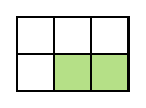
\includegraphics[width=2cm]{fraction2}
 \item 
 
 
\includegraphics[width=1.6cm]{fraction3}
 \item 
 
 \quad 
\includegraphics[width=0.8cm]{fraction4}
 \item 
 
 
\includegraphics[width=1.6cm]{fraction5}
 \item 
 
 
\includegraphics[width=1.5cm]{fraction6}
 \end{colenumerate}
\end{exercice}


\begin{exercice}
Dans quelle(s) figure(s) la surface colorée est‑elle égale au quart de la surface totale ?
\begin{colenumerate}{3}
 \item 
 
 
\includegraphics[width=1.9cm]{fraction7}
  \item 
 
 
\includegraphics[width=1.3cm]{fraction8}
  \item 
 
 
\includegraphics[width=1.3cm]{fraction9}
 \end{colenumerate}
\end{exercice}


\begin{exercice}[Drôles de partages]
Dans quelle(s) figure(s) la surface colorée est‑elle égale au quart de la surface totale ?
\begin{colenumerate}{2}
 \item 
 
 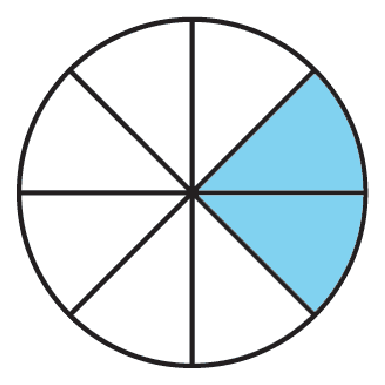
\includegraphics[width=2.1cm]{partage1}
  \item 
 
 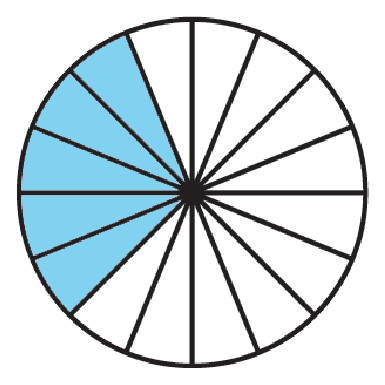
\includegraphics[width=2.1cm]{partage2}
   \item 
 
 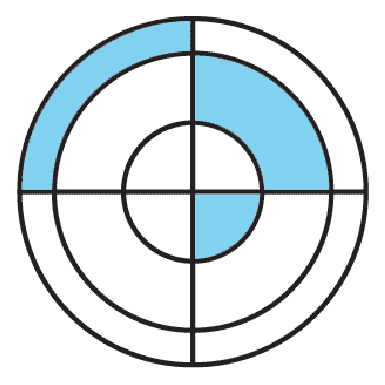
\includegraphics[width=2.1cm]{partage3}
   \item 
 
 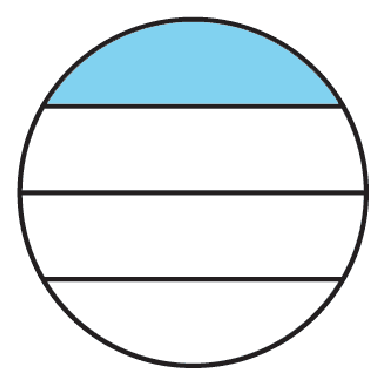
\includegraphics[width=2.1cm]{partage4}
 \end{colenumerate}
\end{exercice}


\begin{exercice}[Avec des quadrilatères]
\begin{enumerate}
  \item Trace un carré de côté 5 cm et colorie trois quarts de sa surface.
  \item Trace un rectangle de largeur 3 cm et de longueur 7 cm. Colorie $\dfrac{7}{21}$ de sa surface.
  \item Trace un carré de côté 3 cm et colorie un sixième de sa surface.
 \end{enumerate}
\end{exercice}


\begin{exercice}[Avec un segment]
\begin{enumerate}
 \item En utilisant le quadrillage de ton cahier, reproduis le segment suivant : \label{NbsRatio_acti10}
 
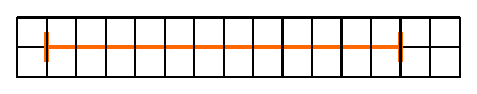
\includegraphics[width=7.9cm]{segment_fraction}
 \item Construis un segment dont la longueur par rapport à celle du segment de la question \ref{NbsRatio_acti10} est :
 \begin{colitemize}{3}
  \item $\dfrac{1}{4}$ ;
  \item $\dfrac{1}{6}$ ;
  \item $\dfrac{5}{4}$.
  \end{colitemize}
 \end{enumerate}
\end{exercice}

%%%%%%%%%%%%%%%%%%%%%%%%%%%%%%%%%%%%%%%%%%%%%%%%%%%%%%%%%%%%%%%%%%%%%%%%

\serie{Différentes écritures}

\begin{exercice}
Donne une écriture fractionnaire des nombres suivants :
\begin{colenumerate}{2}
 \item une demie ;
 \item cinq douzièmes ;
 \item deux tiers ;
 \item sept demis ;
 \item trois quarts ;
 \item cent dix-neuvièmes ;
 \item moins un quart ;
 \item moins trois septièmes.
 \end{colenumerate}
\end{exercice}


\begin{exercice}
Donne une écriture décimale des nombres :
\begin{colenumerate}{2}
 \item deux centièmes ;
 \item quarante dixièmes ;
 \item trois dixièmes ;
 \item cinq-cent millièmes ;
 \item cinq cent‑millièmes ;
 \item neuf tiers ;
 \item moins vingt-deux \newline dixièmes ;
 \item moins cent vingt-trois \newline millièmes.
 \end{colenumerate}
\end{exercice}


\begin{exercice}
Détermine la fraction dont le dénominateur est le numérateur de $\dfrac{41}{17}$ et dont le numérateur est le triple du dénominateur de $\dfrac{53}{9}$.
\end{exercice}


\begin{exercice}
Recopie et complète par deux entiers consécutifs les encadrements suivants :
\begin{colenumerate}{2}
 \item $\ldots < \dfrac{36}{10} < \ldots$ ;
 \item $\ldots < \dfrac{2}{7} < \ldots$ ;
 \item $\ldots < \dfrac{11}{3} < \ldots$ ;
 \item $\ldots < \dfrac{49}{8} < \ldots$ ;
 \end{colenumerate}
\end{exercice}


\begin{exercice}
Recopie et complète par deux entiers consécutifs les encadrements suivants :
\begin{colenumerate}{2}
 \item $\ldots < \dfrac{- 12}{10} < \ldots$ ;
 \item $\ldots < \dfrac{- 18}{7} < \ldots$ ;
 \item $\ldots < \dfrac{-44}{3} < \ldots$ ;
 \item $\ldots < \dfrac{- 35}{8} < \ldots$ ;
 \end{colenumerate}
\end{exercice}


\begin{exercice}
Parmi les fractions suivantes, indique celles qui sont égales à des nombres entiers, puis celles qui sont inférieures à 1 : \\[0.3em]
$\dfrac{42}{10}$ ; $\dfrac{8}{2}$ ; $\dfrac{36}{5}$ ; $\dfrac{1}{6}$ ; $\dfrac{27}{3}$ ; $\dfrac{126}{9}$ ; $\dfrac{87}{2}$ ; $\dfrac{132}{4}$ ; $\dfrac{4}{3}$ ; $\dfrac{33}{42}$.
\end{exercice}


\begin{exercice}
Recopie et complète :
\begin{colenumerate}{3}
 \item $\dfrac{\ldots \ldots}{9} = 1$ ;
 \item $5 = \dfrac{\ldots \ldots}{8}$ ;
 \item $0 = \dfrac{\ldots \ldots}{6}$ ;
 \item $\dfrac{\ldots \ldots}{2} = 4,5$ ;
 \item $\dfrac{1}{\ldots \ldots} = 0,001$ ;
 \item $2,5 = \dfrac{\ldots \ldots}{4}$.
 \end{colenumerate}
\end{exercice}


\begin{exercice}
On considère le quotient $12 : 5$ :
\begin{enumerate}
 \item Donne une écriture fractionnaire de ce quotient. Quel est le numérateur ? Le dénominateur ? \label{NbsRatio_acti11}
 \item Donne une écriture décimale de ce quotient. \label{NbsRatio_acti12}
 \item Reprends les questions \ref{NbsRatio_acti11} et \ref{NbsRatio_acti12} en considérant maintenant le quotient $7 : 8$.
 \end{enumerate}
\end{exercice}


\begin{exercice}
Donne l'écriture décimale de chaque nombre :
\begin{colenumerate}{5}
 \item $\dfrac{1}{8}$ ; 
 \item $\dfrac{46}{5}$ ; 
 \item $\dfrac{56}{70}$ ; 
 \item $\dfrac{11}{16}$ ; 
 \item $\dfrac{153}{12}$.
 \end{colenumerate}
\end{exercice}


%%%%%%%%%%%%%%%%%%%%%%%%%%%%%%%%%%%%%%%%%%%%%%%%%%%%%%%%%%%%%%%%%%%%%%%%

\serie{Demi‑droite graduée}

\begin{exercice}
Donne, sous forme d'une fraction, l'abscisse de chacun des points $A$, $B$ et $C$ placés sur la demi‑droite graduée ci‑dessous :
\begin{center} 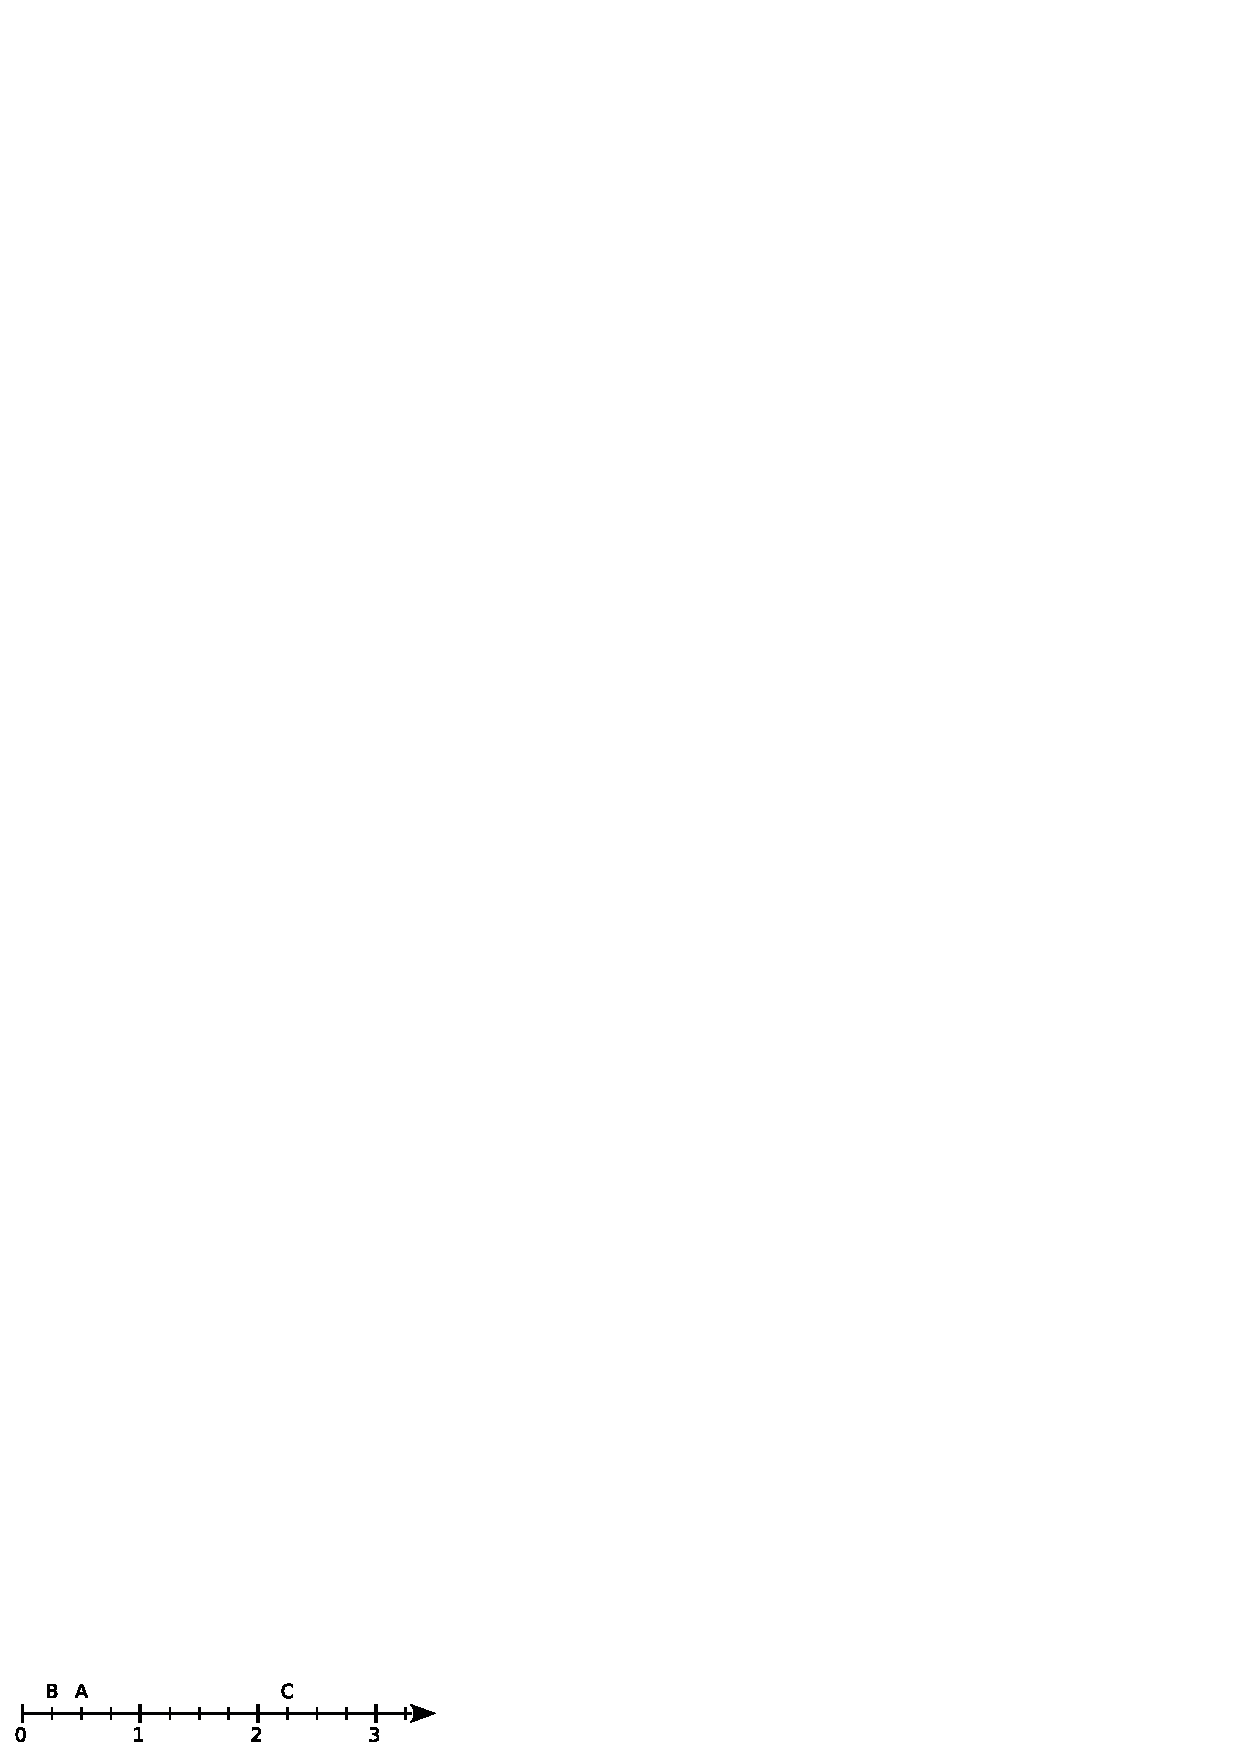
\includegraphics[width=8cm]{dd_BAC03} \end{center}
Donne, sous forme d'une fraction, l'abscisse de chacun des points $R$, $S$ et $T$ placés sur la demi‑droite graduée ci‑dessous :
\begin{center} 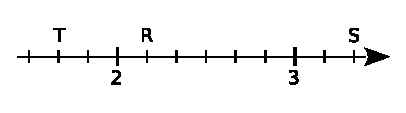
\includegraphics[width=7cm]{dd_TRS23} \end{center}
\end{exercice}


\begin{exercice}
Trace une demi‑droite graduée en prenant 10 cm pour une unité et place les points $M$, $N$, $P$ et $Q$ d'abscisses respectives $\dfrac{3}{10}$ ; 0,7 ; $\dfrac{12}{10}$ et $\dfrac{2}{5}$.
\end{exercice}


\begin{exercice}
Trace une demi‑droite graduée en prenant 10 cm pour une unité et place les points $M$, $N$, $P$ et $Q$ d'abscisses respectives $- \dfrac{7}{10}$ ; $- 0,3$ ; $- \dfrac{2}{10}$ et $- \dfrac{8}{5}$.
\end{exercice}


\begin{exercice}
Trace une demi‑droite graduée en prenant une unité de 3 cm. Place les nombres $\dfrac{5}{3}$ ; $\dfrac{7}{3}$ ; 0,2 ; $\dfrac{4}{5}$ ; $\dfrac{17}{5}$ et 1,5.
\end{exercice}


\begin{exercice}
En choisissant judicieusement la longueur d'une graduation, place précisément sur une demi‑droite graduée les points $A$, $B$, $C$, $D$ et $E$ d'abscisses respectives $\dfrac{5}{12}$, $\dfrac{7}{6}$, $\dfrac{2}{3}$, $\dfrac{3}{2}$ et $\dfrac{5}{4}$.
\end{exercice}


\begin{exercice}
Trace une demi‑droite graduée en prenant 7 cm pour une unité et place les points $E$, $F$ et $G$ d'abscisses respectives $\dfrac{2}{7}$, $1 + \dfrac{3}{7}$ et $1 - \dfrac{4}{7}$.
\end{exercice}


\begin{exercice}
Place précisément sur une demi‑droite graduée les points $U$, $V$ et $W$ d'abscisses respectives $2 + \dfrac{1}{3}$, $6 - \dfrac{2}{3}$ et $3 + \dfrac{4}{3}$.
\end{exercice}

%%%%%%%%%%%%%%%%%%%%%%%%%%%%%%%%%%%%%%%%%%%%%%%%%%%%%%%%%%%%%%%%%%%%%%%%

\serie{Amplifier, simplifier, égalités}

\begin{exercice}[Partage de disques]
En t'inspirant des schémas ci-dessous, écris des égalités de fractions :
\begin{colenumerate}{3}
 \item
 
 
\includegraphics[width=1.5cm]{disque1}
 \item
 
 
\includegraphics[width=1.5cm]{disque2}
 \item
 
 
\includegraphics[width=1.5cm]{disque3}
 \item
 
 
\includegraphics[width=1.5cm]{disque4}
 \item
 
 
\includegraphics[width=1.5cm]{disque5}
 \item
 
 
\includegraphics[width=1.5cm]{disque6}
 \item
 
 
\includegraphics[width=1.5cm]{disque7}
 \item
 
 
\includegraphics[width=1.5cm]{disque8}
 \item
 
 
\includegraphics[width=1.5cm]{disque9}
 \end{colenumerate}
\end{exercice}


\begin{exercice}[Numérateur ou dénominateur fixé]
Recopie et complète :
\begin{colenumerate}{2}
 \item $\dfrac{4}{5} = \dfrac{4 \cdot \ldots}{5 \cdot \ldots} = \dfrac{\ldots}{15}$ ;
 \vspace{0.3cm}
 \item $\dfrac{2}{7} = \dfrac{2 \cdot \ldots}{7 \cdot \ldots} = \dfrac{\ldots}{56}$ ;
 \vspace{0.3cm}
 \item $\dfrac{4}{3} = \dfrac{4 \cdot \ldots}{3 \cdot \ldots} = \dfrac{\ldots}{9}$ ;
 \item $\dfrac{15}{18} = \dfrac{\ldots \cdot \ldots}{6 \cdot \ldots} = \dfrac{\ldots}{6}$ ;
 \item $\dfrac{7}{14} = \dfrac{1 \cdot \ldots}{\ldots \cdot \ldots} = \dfrac{1}{\ldots}$ ;
 \item $\dfrac{12}{20} = \dfrac{\ldots \cdot \ldots}{2 \cdot \ldots} = \dfrac{\ldots}{\ldots}$.
 \end{colenumerate}
\end{exercice}


\begin{exercice}[Numérateur ou dénominateur fixé (bis)]
Recopie et complète :
\begin{colenumerate}{3}
 \item $\dfrac{7}{3} = \dfrac{\ldots}{6}$ ;
 \vspace{0.3cm}
 \item $\dfrac{1}{4} = \dfrac{2}{\ldots}$ ;
 \item $\dfrac{7}{5} = \dfrac{21}{\ldots}$ ;
 \item $\dfrac{3}{4} = \dfrac{\ldots}{100}$ ;
 \item $\dfrac{12}{8} = \dfrac{\ldots}{4}$ ;
 \item $\dfrac{100}{80} = \dfrac{25}{\ldots}$.
 \end{colenumerate}
\end{exercice}


\begin{exercice}[Avec une étape]
Recopie et complète :
\begin{colenumerate}{2}
 \item $\dfrac{10}{6} = \dfrac{\ldots}{3} = \dfrac{25}{\ldots}$ ;
 \vspace{0.3cm}
 \item $\dfrac{12}{15} = \dfrac{\ldots}{5} = \dfrac{8}{\ldots}$ ;
 \vspace{0.3cm}
 \item $\dfrac{27}{18} = \dfrac{\ldots}{2} = \dfrac{15}{\ldots}$ ;
 \item $\dfrac{45}{60} = \dfrac{3}{\ldots} = \dfrac{\ldots}{28}$ ;
 \item $\dfrac{26}{65} = \dfrac{\ldots}{5} = \dfrac{\ldots}{10}$ ;
 \item $\dfrac{49}{42} = \dfrac{7}{\ldots} = \dfrac{\ldots}{72}$.
 \end{colenumerate}
\end{exercice}


\begin{exercice}[Égalités de fractions]
Dans chaque cas, indique, en justifiant, si les fractions données sont égales :
\begin{colenumerate}{2}
 \item $\dfrac{2}{3}$ et $\dfrac{10}{15}$ ;
 \vspace{0.3cm}
 \item $\dfrac{12}{8}$ et $\dfrac{36}{16}$ ;
 \item $\dfrac{12}{15}$ et $\dfrac{4}{5}$ ;
 \item $\dfrac{2}{3}$ et $\dfrac{4}{9}$.
 \end{colenumerate}
\end{exercice}


\begin{exercice}[À la recherche des nombres égaux]
Trouve, parmi les nombres suivants, ceux qui sont égaux :
\begin{colitemize}{3}
 \item $A = \dfrac{7}{4}$ ;
  \vspace{0.2cm}
 \item $B = \dfrac{3}{7}$ ;
   \vspace{0.2cm}
 \item $C = \dfrac{12}{5}$ ;
   \vspace{0.2cm}
 \item $D = \dfrac{9}{49}$ ;
   \vspace{0.2cm}
 \item $E = \dfrac{3}{2}$ ;
   \vspace{0.2cm}
 \item $F = \dfrac{33}{100}$ ;
 \item $G = \dfrac{28}{16}$ ;
 \item $H = \dfrac{1}{3}$ ;
 \item $I = \dfrac{21}{49}$ ;
 \item $J = \dfrac{14}{8}$ ;
 \item $K = 1,5$ ;
 \item $L = \dfrac{18}{12}$ ;
 \item $M = \dfrac{1,2}{0,5}$ ;
 \item $N = \dfrac{15}{10}$ ;
 \item $P = 0,33$ ;
 \item $Q = \dfrac{45}{105}$.
 \end{colitemize}
\end{exercice}


\begin{exercice}[Intrus]
Dans chacune des listes de fractions suivantes se cache un intrus. Trouve-le en justifiant.
\begin{enumerate}
 \item $\dfrac{80}{100}$ ; $\dfrac{16}{20}$ ; $\dfrac{4}{5}$ ; $\dfrac{34}{40}$ ; $\dfrac{8}{10}$ ;
 \vspace{0.2cm}
 \item $\dfrac{12}{16}$ ; $\dfrac{15}{25}$ ; $\dfrac{3}{4}$ ; $\dfrac{75}{100}$ ; $\dfrac{21}{28}$ ;
 \vspace{0.2cm}
 \item $\dfrac{91}{115}$ ; $\dfrac{65}{75}$ ; $\dfrac{130}{150}$ ; $\dfrac{13}{15}$ ; $\dfrac{26}{30}$.
 \end{enumerate}
\end{exercice}


\begin{exercice}[À toi de jouer]
\begin{enumerate}
 \item Trouve quatre fractions égales à $\dfrac{12}{15}$ ;
 \item Trouve cinq fractions égales à $\dfrac{51}{34}$.
 \end{enumerate}
\end{exercice}


\begin{exercice}[Fractions égales]
\begin{enumerate}
 \item Recopie la liste de fractions ci-dessous en regroupant celles qui sont égales : \\[0.5em]
$\dfrac{7}{8}$ ; $\dfrac{5}{2}$ ; $\dfrac{8}{6}$ ; $\dfrac{1}{2}$ ; $\dfrac{4}{3}$ ; $\dfrac{21}{24}$ ; $\dfrac{30}{12}$ ; $\dfrac{12}{9}$ ; $\dfrac{25}{10}$.
\vspace{0.2cm}
 \item Écris cinq fractions égales à $\dfrac{7}{4}$.
 \end{enumerate}
\end{exercice}


\begin{exercice}[Par quoi simplifier ?]
Pour chacune des fractions suivantes, détermine un nombre entier (différent de 1) qui divise à la fois le numérateur et le dénominateur : \\[0.5em]
\begin{colenumerate}{3}
 \item $\dfrac{18}{16}$ ; 
 \vspace{0.2cm}
 \item $\dfrac{5}{10}$ ; 
 \item $\dfrac{12}{22}$ ; 
 \item $\dfrac{27}{9}$ ; 
 \item $\dfrac{60}{36}$ ; 
 \item $\dfrac{84}{35}$.
 \end{colenumerate}
\end{exercice}


\begin{exercice}[Simplification de fractions]
Rends les fractions suivantes irréductibles : \\[0.5em]
\begin{colenumerate}{3}
 \item $\dfrac{6}{4}$ ; 
 \vspace{0.2cm}
 \item $\dfrac{8}{10}$ ; 
 \item $\dfrac{12}{16}$ ; 
 \item $\dfrac{18}{27}$ ; 
 \item $\dfrac{1}{2}$ ; 
 \item $\dfrac{45}{35}$.
 \end{colenumerate}
 \end{exercice}


\begin{exercice}[Simplification de fractions (bis)]
Rends les fractions suivantes irréductibles : \\[0.5em]
\begin{colenumerate}{3}
 \item $\dfrac{13}{7}$ ; 
 \vspace{0.2cm}
 \item $\dfrac{22}{77}$ ; 
 \item $\dfrac{48}{36}$ ; 
 \item $\dfrac{60}{15}$ ; 
 \item $\dfrac{13}{26}$ ; 
 \item $\dfrac{256}{384}$.
 \end{colenumerate}
\end{exercice}


\begin{exercice}[Écriture fractionnaire d'un nombre décimal]
Écris chacun des nombres suivants sous la forme d'une fraction décimale, puis rends irréductible cette fraction :
\begin{colenumerate}{3}
 \item 1,2 ;
 \item 0,6 ;
 \item 2,25 ;
 \item 0,02 ;
 \item 1,125 ;
 \item 1,24.
 \end{colenumerate}
\end{exercice}


\begin{exercice}[D'écriture fractionnaire à fraction]
Transforme chacune des écritures fractionnaires suivantes en une fraction, puis rends irréductible cette fraction :
\begin{colenumerate}{3}
 \item $\dfrac{1,2}{2}$ ; 
 \vspace{0.2cm}
 \item $\dfrac{7,3}{1,5}$ ; 
 \item $\dfrac{1,5}{30}$ ; 
 \item $\dfrac{9,125}{2,5}$ ; 
 \item $\dfrac{7,68}{1,4}$ ; 
 \item $\dfrac{1,3}{7}$.
 \end{colenumerate}
\end{exercice}


\begin{exercice}[De dénominateur 100]
Écris chacun des nombres suivants sous la forme d'une écriture fractionnaire de dénominateur 100 :
\begin{colenumerate}{3}
 \item $\dfrac{1}{2}$ ; 
 \vspace{0.2cm}
 \item $\dfrac{3}{4}$ ; 
 \item $\dfrac{1}{10}$ ; 
 \item $\dfrac{9}{20}$ ; 
 \item $\dfrac{18}{5}$ ; 
 \item 3.
 \end{colenumerate}
\end{exercice}


\begin{exercice}[De fraction à écriture décimale]
Détermine, sans poser de calcul, l'écriture décimale des nombres suivants :
\begin{colenumerate}{4}
 \item $\dfrac{16}{25}$ ; 
 \item $\dfrac{7}{20}$ ; 
 \item $\dfrac{9}{50}$ ; 
 \item $\dfrac{71}{4}$
 \end{colenumerate}
\end{exercice}

%%%%%%%%%%%%%%%%%%%%%%%%%%%%%%%%%%%%%%%%%%%%%%%%%%%%%%%%%%%%%%%%%%%%%%%%

\serie{Comparer, ordonner}

\begin{exercice}[Comparer des fractions à des entiers]
\begin{enumerate}
 \item Recopie les fractions suivantes puis entoure en vert celles qui sont inférieures à 1 et en rouge celles qui sont supérieures à 1 : \\[0.5em]
 $\dfrac{7}{8}$ ;  $\dfrac{9}{4}$ ;  $\dfrac{12}{5}$ ;  $\dfrac{634}{628}$ ;  $\dfrac{9}{10}$ ;  $\dfrac{18}{8}$ ;  $\dfrac{182}{196}$ ;  $\dfrac{4}{23}$.
 \vspace{0.2cm}
 \item Recopie puis entoure les fractions inférieures à 2 en expliquant ta démarche : \\[0.5em]
 $\dfrac{64}{21}$ ;  $\dfrac{35}{18}$ ;  $\dfrac{41}{18}$ ;  $\dfrac{12}{25}$ ;  $\dfrac{14}{30}$ ;  $\dfrac{169}{83}$ ;  $\dfrac{1}{2}$ ;  $\dfrac{12}{25}$.
 \end{enumerate}
\end{exercice}


\begin{exercice}
Recopie en remplaçant les points de suspension par les symboles $<$ ou $>$ :
\begin{colenumerate}{3}
 \item $\dfrac{4}{5} \ldots \dfrac{7}{5}$ ; 
 \vspace{0.2cm}
 \item $\dfrac{2}{13} \ldots \dfrac{1}{13}$ ; 
 \item $\dfrac{19}{23} \ldots \dfrac{31}{23}$ ; 
 \item $\dfrac{7}{6} \ldots \dfrac{3}{6}$ ; 
 \item $\dfrac{21}{9} \ldots \dfrac{31}{9}$ ; 
 \item $\dfrac{15}{3} \ldots \dfrac{12}{3}$.
 \end{colenumerate}
\end{exercice}


\begin{exercice}
Recopie en remplaçant les points de suspension par les symboles $<$ ou $>$ :
\begin{colenumerate}{3}
 \item $\dfrac{1}{2} \ldots \dfrac{1}{4}$ ; 
 \vspace{0.2cm}
 \item $\dfrac{7}{5} \ldots \dfrac{7}{6}$ ; 
 \item $\dfrac{41}{51} \ldots \dfrac{41}{49}$ ; 
 \item $\dfrac{62}{41} \ldots \dfrac{62}{35}$ ; 
 \item $\dfrac{12}{6} \ldots \dfrac{12}{18}$ ; 
 \item $5 \ldots \dfrac{5}{2}$.
 \end{colenumerate}
\end{exercice}


\begin{exercice}
Recopie en remplaçant les points de suspension par les symboles < ou >. Justifie tes réponses :
\begin{colenumerate}{3}
 \item $\dfrac{2}{3} \ldots \dfrac{1}{9}$ ; 
 \vspace{0.2cm}
 \item $\dfrac{1}{2} \ldots \dfrac{1}{4}$ ; 
 \item $\dfrac{3}{4} \ldots \dfrac{7}{8}$ ; 
 \item $\dfrac{12}{15} \ldots \dfrac{4}{3}$ ; 
 \item $\dfrac{7}{18} \ldots \dfrac{3}{9}$ ; 
 \item $\dfrac{19}{10} \ldots \dfrac{10}{5}$.
 \end{colenumerate}
\end{exercice}


\begin{exercice}
Comparer puis vérifier :
\begin{enumerate}
  \item Compare $\dfrac{7}{5}$ et $\dfrac{22}{15}$ ;
  \item Compare $\dfrac{13}{9}$ et $\dfrac{4}{3}$ ;
  \item Avec une calculatrice, donne une valeur approchée de chacune des fractions et vérifie tes réponses.
 \end{enumerate}
\end{exercice}


\begin{exercice}
Recopie en remplaçant les points de suspension par les symboles <, > ou =. Justifie tes réponses :
\begin{colenumerate}{3}
 \item $\dfrac{4}{7} \ldots \dfrac{7}{14}$ ; 
 \vspace{0.2cm}
 \item $\dfrac{7}{8} \ldots \dfrac{16}{15}$ ;
 \vspace{0.2cm}
 \item $\dfrac{13}{4} \ldots \dfrac{27}{8}$ ; 
 \item $\dfrac{12}{15} \ldots \dfrac{12}{14}$ ; 
 \item $\dfrac{9}{18} \ldots \dfrac{3}{6}$ ; 
 \item $\dfrac{24}{10} \ldots \dfrac{10}{5}$ ; 
 \item $\dfrac{7}{84} \ldots \dfrac{1}{12}$ ; 
 \item $\dfrac{6}{5} \ldots \dfrac{6}{4}$ ; 
 \item $\dfrac{7}{4} \ldots 2$.
 \end{colenumerate}
\end{exercice}


\begin{exercice}[De l'ordre !]
\begin{enumerate}
 \item Trouve une méthode permettant de ranger ces fractions dans l'ordre croissant : \\[0.1em]
 \begin{center} $\dfrac{3}{16}$ ; $\dfrac{1}{4}$ ; $\dfrac{7}{8}$ ; $\dfrac{3}{2}$ ; $\dfrac{9}{16}$ ; $\dfrac{8}{4}$ ; $\dfrac{1}{2}$. \end{center}
 \vspace{0.2cm}
 \item Trouve une méthode permettant de ranger ces fractions dans l'ordre croissant : \\[0.1em]
 \begin{center} $\dfrac{16}{3}$ ; $\dfrac{4}{1}$ ; $\dfrac{8}{7}$ ; $\dfrac{2}{3}$ ; $\dfrac{16}{9}$ ; $\dfrac{4}{8}$ ; $\dfrac{2}{1}$. \end{center}
 \end{enumerate}
\end{exercice}


\begin{exercice}[Avec un axe]
\begin{enumerate}
 \item Range ces fractions dans l'ordre décroissant : \\[0.1em] \label{NbsRatio_approf1}
\begin{center} $\dfrac{2}{3}$ ; $\dfrac{5}{6}$ ; $\dfrac{1}{6}$ ; $\dfrac{7}{12}$ ; $\dfrac{4}{3}$ ; $\dfrac{13}{6}$ ; $\dfrac{5}{3}$. \end{center}
 \vspace{0.2cm}
 \item Trace un axe gradué d'unité douze carreaux. Place les fractions précédentes.
 \item Vérifie que ton classement de la question \ref{NbsRatio_approf1} est correct.
 \end{enumerate}
\end{exercice}


\begin{exercice}[Un autre exo]
Dans chaque cas, réponds à la question en comparant deux fractions :
\begin{enumerate}
 \item Le cirque Pandor possède douze animaux dont cinq des fauves. Le cirque Zopoutou possède vingt-quatre animaux dont onze fauves. Quel cirque a la plus grande proportion de fauves ?
 \item Dans les parkings, la loi exige que sur 50 places, au moins une soit réservée aux personnes handicapées. Un parking de 600 places met à disposition 10 places pour handicapés. Ce parking respecte-t-il la loi ?
 \item Mon frère a déjà fait 60 parties sur le jeu "Robostrike". Il a gagné 33 fois. Pour ma part, je joue depuis plus longtemps. J'ai déjà 300 parties à mon actif dont 153 victoires. Est-ce qu'on peut dire que je gagne plus souvent que mon frère ?
 \item J'ai eu deux notes en maths : trois points sur cinq et onze points sur vingt. Quelle est le meilleur de ces deux tests ? 
 \end{enumerate}
\end{exercice}


\begin{exercice}[Intercaler]
Dans chaque cas, trouve deux fractions comprises entre :
\begin{colenumerate}{3}
 \item $\dfrac{2}{3}$ et $\dfrac{5}{3}$ ; 
 \vspace{0.2cm}
 \item $\dfrac{12}{30}$ et $\dfrac{20}{30}$ ; 
 \item $\dfrac{4}{7}$ et $\dfrac{5}{7}$ ; 
 \item $3$ et $3,1$ ; 
 \item $12$ et $\dfrac{61}{5}$ ; 
 \item $- \dfrac{32}{5}$ et $- \dfrac{13}{2}$.
 \end{colenumerate}
\end{exercice}

%%%%%%%%%%%%%%%%%%%%%%%%%%%%%%%%%%%%%%%%%%%%%%%%%%%%%%%%%%%%%%%%%%%%%%%%

\serie{Prendre une fraction d'un nombre}

\begin{exercice}[Astucieusement]
\begin{enumerate}
 \item Quelle méthode est la plus astucieuse pour effectuer le calcul $\dfrac{3}{4} \cdot 16$? Justifie ta réponse.
 \item Effectue les calculs suivants sans calculatrice le plus astucieusement possible :
 \begin{colitemize}{3}
  \item $\dfrac{21}{3} \cdot 5$ ;
  \vspace{0.2cm}
  \item $\dfrac{35}{4} \cdot 12$ ;
  \item $\dfrac{18}{7} \cdot 14$ ;
  \item $3,4 \cdot \dfrac{5}{17}$ ;
  \item $\dfrac{8}{16} \cdot 4,28$ ;
  \item $\dfrac{7}{3} \cdot 36,9$ ;
  \end{colitemize}
 \end{enumerate}
\end{exercice}


\begin{exercice}
Traduis chaque énoncé par un calcul que tu effectueras :
\begin{enumerate}
 \item Le quart de cent ;
 \item Les trois quarts de soixante ;
 \item Les cinq tiers de trois cent soixante ;
 \item Quatre‑vingts centièmes de trente.
 \end{enumerate}
\end{exercice}


\begin{exercice}
Recopie et complète :
 \begin{colenumerate}{2}
  \item $\ldots \cdot \dfrac{8}{7} = \dfrac{56}{7}$ ;
  \vspace{0.2cm}
  \item $\dfrac{7}{5} \cdot \ldots = \dfrac{42}{5}$ ;
  \vspace{0.2cm}
  \item $\dfrac{9 \cdot \ldots}{11} = \dfrac{72}{11}$ ;
  \item $\ldots \cdot \dfrac{8}{7} = 16$ ;
  \item $\dfrac{9}{14} \cdot \ldots = \dfrac{27}{7}$ ;
  \item $\dfrac{\ldots \cdot 5}{20} = \dfrac{3}{4}$.
 \end{colenumerate}
\end{exercice}


\begin{exercice}
Pour chaque question, dis si les nombres donnés sont égaux :
\begin{enumerate}
 \item Trois quarts de seize et $6 \cdot \dfrac{48}{24}$ ;
 \item Deux cinquièmes de vingt et $\dfrac{2}{3} \cdot 12$ ;
 \item Cinq douzièmes de trente-deux et $4,2 \cdot \dfrac{33}{11}$.
 \end{enumerate}
\end{exercice}


\begin{exercice}[Multiplication par 0,1 ; 0,01 ; 0,001]
\begin{enumerate}
 \item Recopie et complète : \\[0.2em]
$578,4 \cdot 0,01 = 578,4 \cdot \dfrac{1}{\ldots} = \dfrac{578,4 \cdot \ldots}{\ldots} = \dfrac{\ldots}{\ldots} = \ldots$ ;
\vspace{0.2cm}       
 \item Sur le même modèle, effectue les calculs :
 \begin{colitemize}{3}
  \item $89,3 \cdot 0,1$ ;
  \item $0,12 \cdot 0,001$ ;
  \item $890\,001 \cdot 0,01$.  
  \end{colitemize}
 \end{enumerate}
\end{exercice}


\begin{exercice}[Avec la calculatrice]
À l'aide de la calculatrice, trouve le résultat des calculs suivants (précise si le résultat est exact ou approché) :
\begin{enumerate}
 \item $25\,361 \cdot \dfrac{84}{521}$ ;
 \vspace{0.2cm}
 \item $17\,232 \cdot \dfrac{591}{48}$.
 \end{enumerate}
\end{exercice}


\begin{exercice}[Pourcentages de base]
Calcule :
\begin{colenumerate}{2}
 \item 25 \% de 100 g ;
 \item 30 \% de 200 m ;
 \item 70 \% de 15 CHF ;
 \item 150 \% de 15 kg.
 \end{colenumerate}
\end{exercice}


\begin{exercice}[Combien de minutes ?]
\begin{enumerate}
 \item Exprime en minutes, en justifiant, chacune des durées suivantes :
 \begin{itemize}
  \item une demi‑heure ;
  \item deux tiers d'une heure ;
  \item trois quarts d'heure ;
  \item une heure et quart.
  \end{itemize}
 \item Transforme les durées suivantes en heures et minutes :
 \begin{colitemize}{2}
  \item sept quarts d'heure;
  \item un vingtième d'heure ;
  \item neuf demi‑heures ;
  \item six dixièmes d'heure.
  \end{colitemize}
 \end{enumerate}
\end{exercice}


\begin{exercice}[Partage d'un segment]
Trace un segment $[AB]$ de 63 mm.

Place un point $C$ appartenant à $[AB]$ tel que $[AC]$ mesure les $\dfrac{5}{7}$ de $[AB]$.
\end{exercice}


\begin{exercice}[Le partage]
Hugo a 43,20 CHF dans sa tirelire. Il décide d'en donner les $\dfrac{4}{9}$ à son petit frère Lukas. Combien Lukas va-t-il recevoir ?
\end{exercice}


\begin{exercice}[Le cycliste]
Un cycliste fait un trajet de 45 km dont les deux tiers sont en montée. Quelle est la longueur de la montée ?
\end{exercice}


\begin{exercice}[Le réservoir]
Le réservoir de ma voiture a une capacité de 56 litres. Il est rempli aux $\dfrac{3}{14}$ d'essence. Combien reste‑t‑il de litres d'essence dans ce réservoir ?
\end{exercice}


\begin{exercice}[Les élèves de sixième]
252 élèves de sixième ont été interrogés sur la fréquence hebdomadaire de leur pratique du sport en dehors de l'école. \\[0.2em]
\begin{itemize}
 \item $\dfrac{1}{6}$ des élèves ne pratique aucun sport ;
 \vspace{0.2cm}
 \item $\dfrac{3}{7}$ des élèves en font une fois ;
 \vspace{0.2cm}
 \item $\dfrac{3}{14}$ des élèves en font deux fois ;
 \vspace{0.2cm}
 \item Le reste des élèves en fait plus de deux fois par semaine. Calcule le nombre d'élèves pour chaque catégorie.
 \end{itemize}
\end{exercice}


\begin{exercice}[Au cinéma]
Dans la grande salle de 175 places d'un cinéma de quartier, est projeté un film qui a permis de remplir la salle à 76 \%. Combien y a‑t‑il eu de spectateurs à cette séance ?
\end{exercice}


\begin{exercice}[Composition d'un aliment]
Un plat préparé de 254 g contient 27 \% de lipides, 55 \% de protides et 16 \% de glucides. 
Détermine la masse de ces trois substances dans ce plat.
\end{exercice}


\begin{exercice}[L'air]
L'air est constitué principalement d'azote et d'oxygène. Dans un volume d'air donné, le volume d'azote correspond à 78,6 \% du volume total et celui d'oxygène à 20,9 \%. Sachant qu'une salle de classe a un volume de 125 m\up{3}, calcule le volume, en m\up{3}, de chacun de ces gaz présents dans cette salle.
\end{exercice}


\begin{exercice}[Du chocolat blanc]
Le chocolat blanc contient 20 \% de beurre de cacao, 14 \% de matière sèche d'origine lactique et 55 \% de sucre. \\[0.5em]
Calcule la masse de chacun de ces ingrédients dans une tablette de chocolat blanc de 150 g.
\end{exercice}


%%%%%%%%%%%%%%%%%%%%%%%%%%%%%%%%%%%%%%%%%%%%%%%%%%%%%%%%%%%%%%%%%%%%%%%%

\serie{Additionner, soustraire}

\begin{exercice}
L'égalité $\dfrac{1}{3} + \dfrac{7}{12} = \dfrac{11}{12}$ est illustrée par la figure ci-dessous :
\begin{center} 
\includegraphics[width=1.7cm]{addition_fraction1} \end{center}
\begin{enumerate}
 \item Explique pourquoi. \label{NbsRatio_entrain2}
 \item En t'inspirant de la question \ref{NbsRatio_entrain2}, écris une égalité illustrant chacune des figures suivantes :
 
 \begin{minipage}[t]{0.28\linewidth}
 \begin{center} Figure 1 \end{center}
 \begin{center} 
\includegraphics[width=1.1cm]{addition_fraction2} \end{center}
  \end{minipage} \hfill%
 \begin{minipage}[t]{0.38\linewidth}
 \begin{center} Figure 2 \end{center}
 \begin{center} 
\includegraphics[width=2.6cm]{addition_fraction3} \end{center}
  \end{minipage} \hfill%
 \begin{minipage}[t]{0.3\linewidth}
 \begin{center} Figure 3 \end{center}
 \begin{center} 
\includegraphics[width=2.1cm]{addition_fraction4} \end{center}
  \end{minipage} \\
 \end{enumerate}
\end{exercice}


\begin{exercice}
Effectue les opérations suivantes et donne le résultat sous la forme d'une fraction irréductible : \\[0.1em]
\begin{colenumerate}{3}
 \item $\dfrac{7}{9} + \dfrac{5}{9}$ ;
 \vspace{0.2cm}
 \item $\dfrac{19}{8} - \dfrac{15}{8}$ ;
 \item $\dfrac{5}{12} + \dfrac{13}{12}$ ;
 \item $\dfrac{9}{11} + \dfrac{7}{11}$ ;
 \item $\dfrac{7}{18} + \dfrac{11}{18}$ ;
  \item $\dfrac{27}{13} - \dfrac{1}{13}$.
 \end{colenumerate}
\end{exercice}


\begin{exercice}
Effectue les opérations suivantes : \\[0.1em]
\begin{colenumerate}{3}
 \item $\dfrac{2}{13} + \dfrac{7}{13}$ ;
 \vspace{0.2cm}
 \item $\dfrac{8}{7} - \dfrac{6}{7}$ ;
 \vspace{0.2cm}
 \item $\dfrac{9}{4} - \dfrac{5}{12}$ ;
 \item $\dfrac{1}{2} + \dfrac{1}{4}$ ;
 \item $\dfrac{1}{3} - \dfrac{1}{6}$ ;
 \item $\dfrac{13}{14} + \dfrac{5}{7}$ ;
 \item $\dfrac{2}{3} - \dfrac{1}{18}$ ;
 \item $\dfrac{8}{5} - \dfrac{16}{10}$ ;
  \item $\dfrac{5}{6} + \dfrac{5}{12}$.
 \end{colenumerate}
\end{exercice}


\begin{exercice}
Effectue les opérations suivantes : \\[0.1em]
\begin{colenumerate}{3}
 \item $4 - \dfrac{3}{2}$ ;
 \vspace{0.2cm}
 \item $2 + \dfrac{1}{3}$ ;
 \vspace{0.2cm}
 \item $\dfrac{9}{4} - 1$ ;
 \item $7 + \dfrac{1}{4}$ ;
 \item $\dfrac{16}{3} - 3$ ;
 \item $4 + \dfrac{5}{7}$ ;
 \item $6 - \dfrac{5}{3} - \dfrac{5}{6}$ ;
 \item $2 + \dfrac{3}{4} + \dfrac{7}{2}$ ;
  \item $7 - \dfrac{9}{5} - \dfrac{13}{25}$.
 \end{colenumerate}
\end{exercice}


\begin{exercice}
Effectue les opérations suivantes : \\[0.1em]
\begin{colenumerate}{3}
 \item $\dfrac{4}{21} + \dfrac{1}{3}$ ;
 \vspace{0.2cm}
 \item $\dfrac{2}{7} - \dfrac{6}{35}$ ;
 \vspace{0.2cm}
 \item $\dfrac{9}{80} - \dfrac{1}{10}$ ;
 \item $\dfrac{1}{8} + \dfrac{5}{56}$ ;
 \item $\dfrac{3}{2} + \dfrac{1}{5}$ ;
 \item $\dfrac{4}{3} + \dfrac{5}{7}$ ;
 \item $\dfrac{1}{5} - \dfrac{1}{4}$ ;
 \item $\dfrac{4}{15} - \dfrac{3}{2}$ ;
  \item $\dfrac{1}{6} + 1$.
 \end{colenumerate}
\end{exercice}


\begin{exercice}
Dans chacun des cas suivants, calcule la valeur de $a + b -  c$ : 
\begin{enumerate}
 \item $a = \dfrac{1}{2}$ ; $b = \dfrac{3}{4}$ ; $c = \dfrac{1}{4}$ ;
  \vspace{0.2cm}
 \item $a = \dfrac{7}{6}$ ; $b = \dfrac{10}{3}$ ; $c = \dfrac{5}{6}$ ;
  \vspace{0.2cm}
 \item $a = \dfrac{1}{3}$ ; $b = \dfrac{1}{9}$ ; $c = \dfrac{1}{27}$ ;
  \vspace{0.2cm}
 \item $a = \dfrac{2}{5}$ ; $b = \dfrac{13}{15}$ ; $c = \dfrac{2}{5}$.
 \end{enumerate}
\end{exercice}


\begin{exercice}[Étonnant !]
\begin{enumerate}
 \item Calcule : $\dfrac{1}{2} + \dfrac{1}{4}$ ;
  \vspace{0.2cm}
 \item Calcule : $\dfrac{1}{2} + \dfrac{1}{4} + \dfrac{1}{8}$ ;
  \vspace{0.2cm}
 \item Calcule : $\dfrac{1}{2} + \dfrac{1}{4} + \dfrac{1}{8} + \dfrac{1}{16}$ ;
  \vspace{0.2cm}
 \item Sans calculer, essaie de deviner la valeur de $\dfrac{1}{2} + \dfrac{1}{4} + \dfrac{1}{8} + \dfrac{1}{16} + \dfrac{1}{32} + \dfrac{1}{64}$ puis vérifie.
 \end{enumerate}
\end{exercice}


\begin{exercice}
Jimmy a mangé $\dfrac{1}{4}$ d'un gâteau. Élise a mangé $\dfrac{3}{8}$ du même gâteau.
\begin{enumerate}
 \item Quelle part du gâteau ont-ils mangée à eux deux ?
 \item Quelle part du gâteau reste-t-il ?
 \end{enumerate}
\end{exercice}


\begin{exercice}[Jeu vidéo]
Trois frères veulent acheter ensemble un jeu vidéo. Le premier ne possède que les $\dfrac{3}{5}$ du prix de ce jeu vidéo, le deuxième n'en possède que les $\dfrac{4}{15}$ et le troisième seulement $\dfrac{1}{3}$. 
\begin{enumerate}
 \item Ont-ils assez d'argent pour acheter ce jeu vidéo ?
 \item Peuvent-ils acheter un second jeu vidéo de même prix ?
 \end{enumerate}
\end{exercice}


\begin{exercice}[Triangle]
$ABC$ est un triangle isocèle en $A$ tel que $AB = \dfrac{5}{7}\,\,BC$ . Quelle fraction de $BC$ représente son périmètre ?
\end{exercice}


\begin{exercice}[Pyramide]
Recopie puis complète la pyramide suivante sachant que le nombre contenu dans une case est la somme des nombres contenus dans les deux cases situées en dessous de lui :
\begin{center} $\boxed{\phantom{\dfrac{16}{42} \dfrac{16}{42} \dfrac{16}{42}}}$ \end{center}
\vspace{-0.72cm}
\begin{center} \boxed{\phantom{\dfrac{16}{42} \dfrac{16}{42} \dfrac{16}{42}}} \negthinspace \boxed{\phantom{\dfrac{16}{42} \dfrac{16}{42} \dfrac{16}{42}}} \end{center}
\vspace{-0.8cm}
\begin{center} \boxed{\phantom{\dfrac{16}{42} \dfrac{16}{42} \dfrac{16}{42}}} \negthinspace \boxed{\phantom{\dfrac{16}{42}} \dfrac{16}{42} \phantom{\dfrac{16}{42}}} \negthinspace  \boxed{\phantom{\dfrac{16}{42} \dfrac{16}{42} \dfrac{16}{42}}} \end{center}
\vspace{-0.79cm}
\begin{center} \negthinspace \boxed{\phantom{!\dfrac{16}{42}} \dfrac{1}{3} \phantom{!\dfrac{16}{42}}} \negthinspace \boxed{\phantom{\dfrac{16}{42}} \dfrac{1}{21} \phantom{\dfrac{16}{42}}} \negthinspace \boxed{\phantom{\dfrac{16}{42} \dfrac{16}{42} \dfrac{16}{42}}} \negthinspace \boxed{\phantom{!\dfrac{16}{42}} \dfrac{2}{3} \phantom{!\dfrac{16}{42}}} \end{center}
\vspace{-0.69cm}
\end{exercice}

%%%%%%%%%%%%%%%%%%%%%%%%%%%%%%%%%%%%%%%%%%%%%%%%%%%%%%%%%%%%%%%%%%%%%%%%
\end{colonne*exercice}


\exercicesappr
\begin{colonne*exercice}
\begin{exercice}[Quelques partages]
Pour chaque figure, indique la fraction de la surface totale qui est colorée :
\begin{colenumerate}{3}
 \item 
 
 
\includegraphics[width=2cm]{partages_colores}
 \item
  
 
\includegraphics[width=2cm]{partages_colores2}
 \item
  
 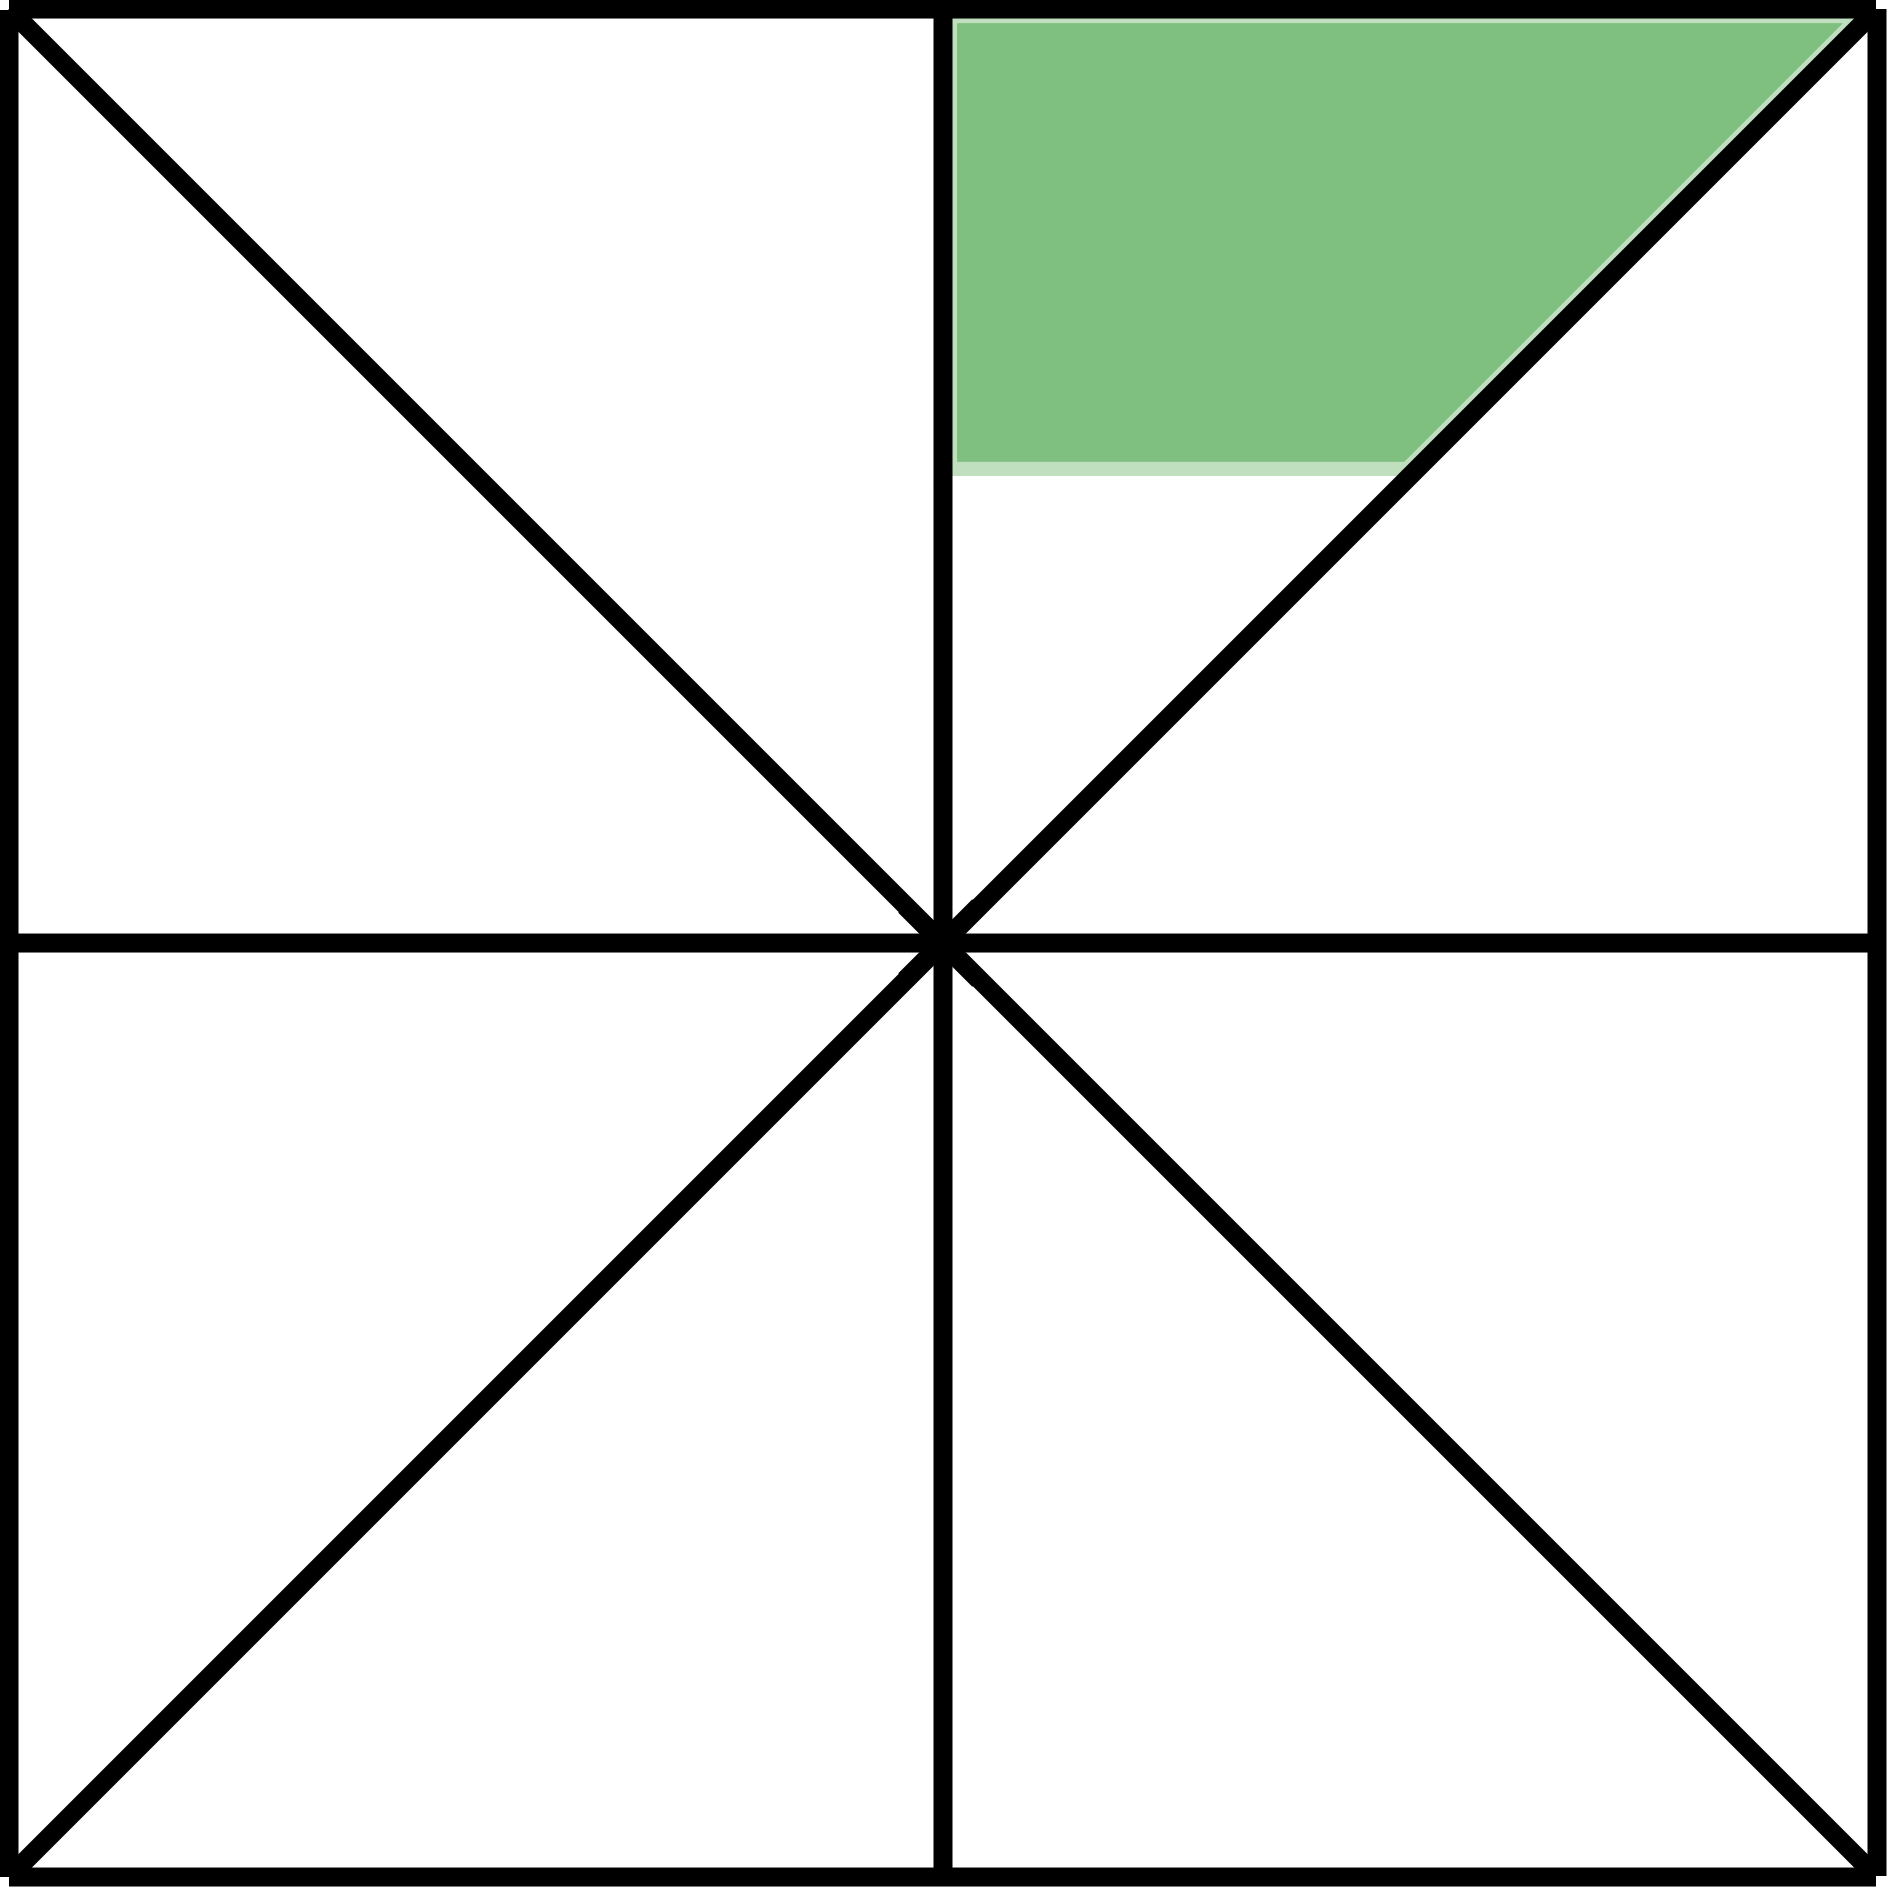
\includegraphics[width=2cm]{partages_colores3}
 \end{colenumerate}
\end{exercice}


\begin{exercice}[Coloriage]
Trace trois rectangles de 9 cm sur 4 cm.
\begin{enumerate}
 \item Partage le premier pour colorier les cinq sixièmes de sa surface ;
 \item Partage le second pour colorier les sept douzièmes de sa surface ;
 \item Partage le troisième pour colorier les trois huitièmes de sa surface.
 \end{enumerate}
\end{exercice}


\begin{exercice}
Transforme les nombres suivants en écriture décimale puis entoure d’une même couleur ceux qui sont égaux :
\begin{center}
\renewcommand{\arraystretch}{2}
  \begin{tabular}{|c|c|c|c|c|c|} 
  \hline
  \rowcolor{F2} $7 + \dfrac{1}{4}$ & 2 & $\dfrac{29}{4}$ & $\dfrac{156}{78}$ & $\dfrac{84}{10}$ & 29,4 \\\hline
  \rowcolor{F2} $8 - \dfrac{3}{4}$ & 8,4 & $\dfrac{8}{4}$ & $8 + \dfrac{4}{10}$ & $\dfrac{147}{5}$ & 7,25 \\\hline
  \end{tabular}
  \renewcommand{\arraystretch}{1}
 \end{center}
\end{exercice}


\begin{exercice}[À la chasse aux décimaux]
\begin{enumerate}
 \item Parmi les fractions suivantes, lesquelles sont des nombres décimaux ?
 \begin{colitemize}{4}
  \item $A = \dfrac{1}{2}$ ;
  \item $B = \dfrac{1}{3}$ ;
  \item $C = \dfrac{1}{7}$ ;
  \item $D = \dfrac{1}{10}$ ;
  \item $E = \dfrac{1}{13}$ ;
  \item $F = \dfrac{1}{25}$ ;
  \item $G = \dfrac{1}{16}$ ;
  \item $H = \dfrac{1}{12}$ ;
  \item $I = \dfrac{1}{4}$ ;
  \item $J = \dfrac{1}{15}$.
  \end{colitemize}
Tu pourras utiliser un tableau pour présenter tes résultats.
 \item Donne deux fractions de numérateur 1 (différentes des fractions ci-dessus) : une  décimale et une non décimale.
 \item Quelles remarques peux-tu faire concernant les fractions décimales ?
 \item Sans calculer les quotients, indique si les fractions suivantes sont décimales ou non, en justifiant ta réponse : $\dfrac{1}{125}$ ; $\dfrac{1}{40}$ ; $\dfrac{1}{6}$ et $\dfrac{1}{35}$.
 \vspace{0.2cm}
 \item Soulimane affirme que toute fraction décimale peut s'écrire avec un dénominateur égal à 10, 100, 1\,000 \ldots
 
 Est-ce vrai ?
 \end{enumerate}
\end{exercice}


\begin{exercice}[Demi‑droites graduées]
\begin{enumerate}
 \item Quelles sont les abscisses respectives des points $A$, $B$, $C$ et $D$ ?
 
 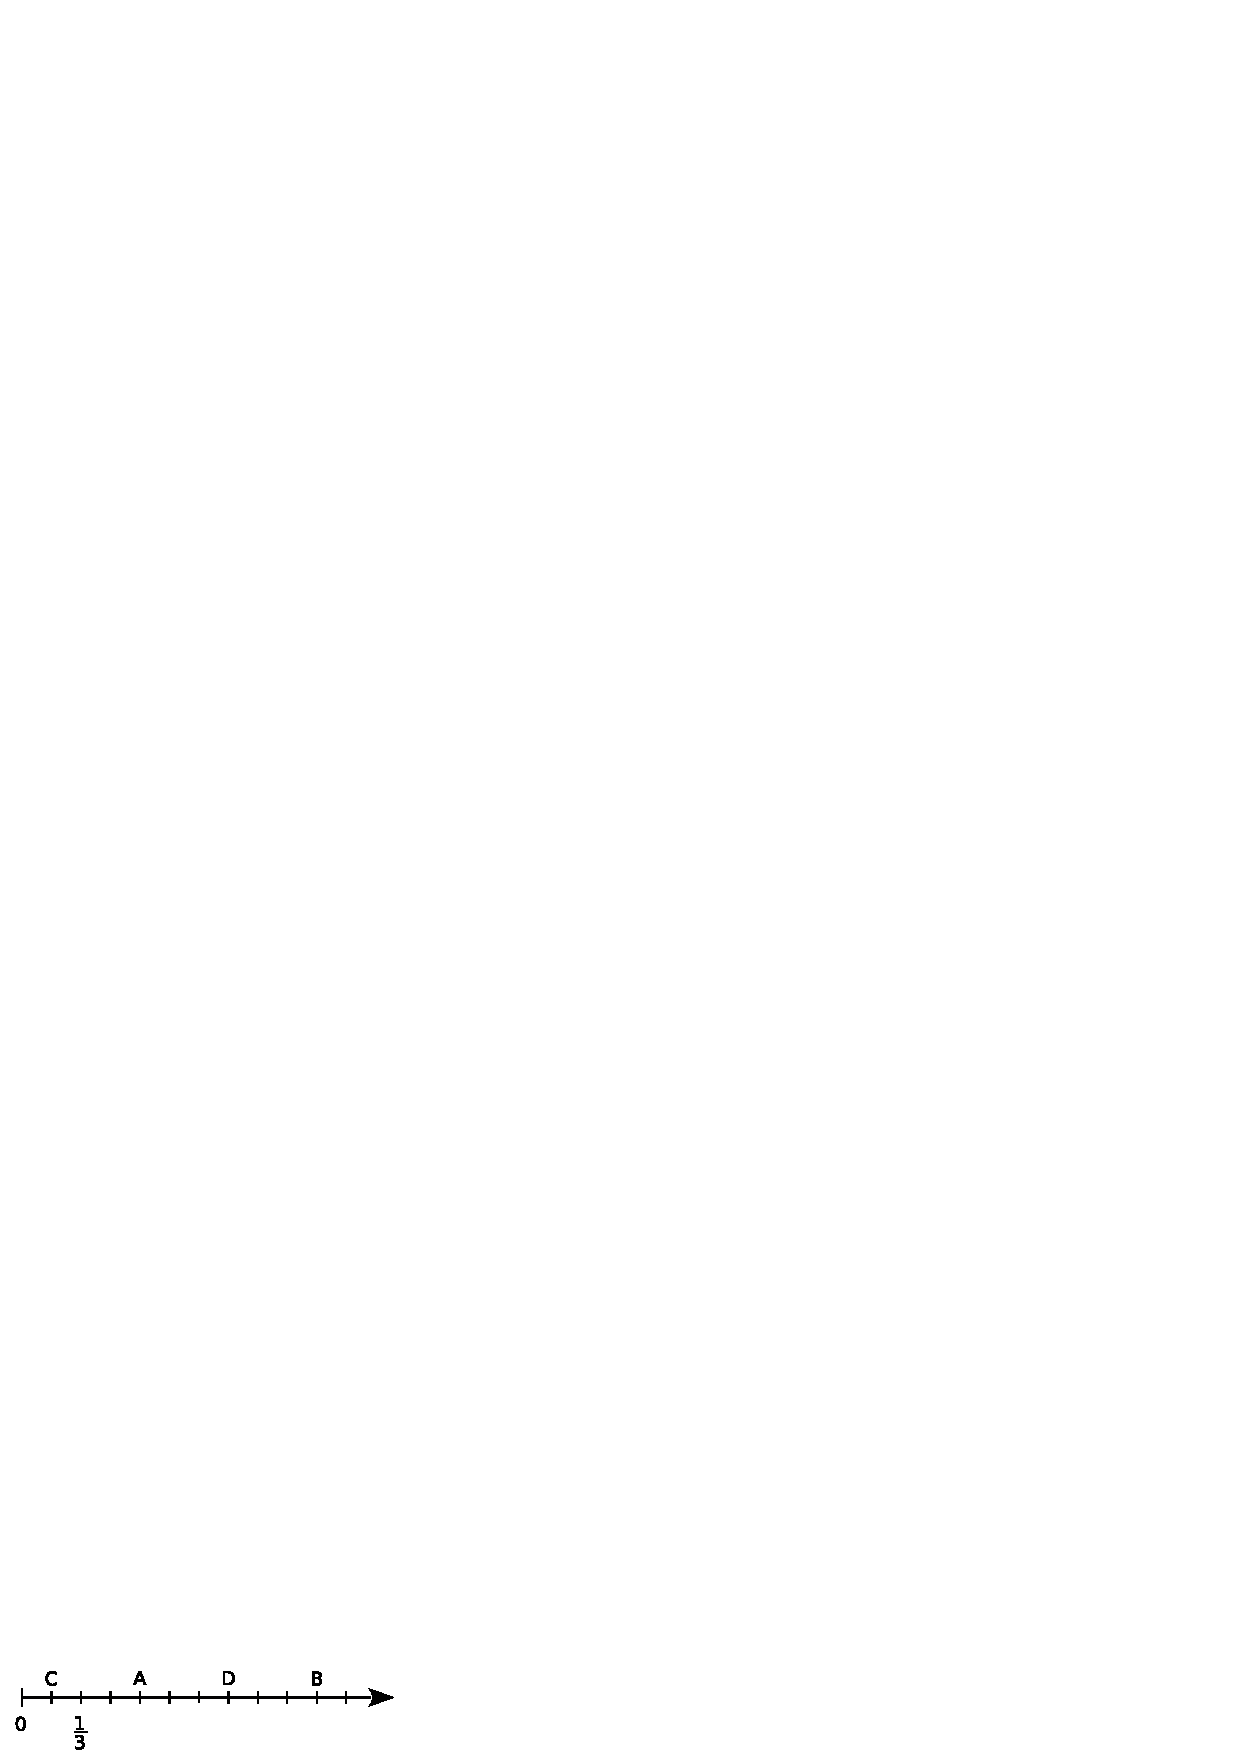
\includegraphics[width=6.7cm]{dd_fraction1}
 \item Même question pour les points $E$, $F$, $G$ et $H$.
 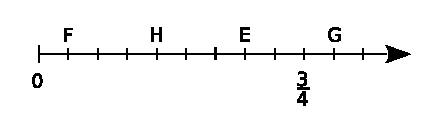
\includegraphics[width=6.7cm]{dd_fraction2}
 \item Même question pour les points $I$, $J$, $K$ et $L$.
 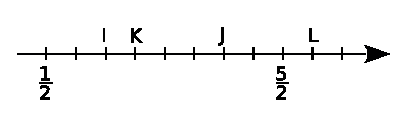
\includegraphics[width=6.7cm]{dd_fraction3}
 \item Même question pour les points $P$, $M$ et $N$.
 \includegraphics[width=6.7cm]{dd_fraction4}
 \end{enumerate}
\end{exercice}


\begin{exercice}
En choisissant judicieusement une unité de longueur, place précisément sur une demi‑droite graduée les points $A$ d'abscisse $\dfrac{5}{6}$, $B$ d'abscisse $\dfrac{1}{2}$, C d'abscisse $\dfrac{11}{6}$, D d'abscisse $\dfrac{3}{4}$ et E d'abscisse $1 + \dfrac{1}{3}$.
\end{exercice}


\begin{exercice}[Encore une demi‑droite graduée]
\begin{enumerate}
 \item Reproduis la demi‑droite graduée ci‑dessous en prenant trois centimètres pour unité :
 \includegraphics[width=6.7cm]{dd_PMN}
 \item Donne deux écritures de chacune des abscisses des points $M$, $N$ et $P$.
 \item Sur la demi‑droite graduée, place le point $Q$ d'abscisse $14 + \dfrac{1}{3}$, le point $R$ d'abscisse $13 - \dfrac{1}{6}$ et le point $S$ d'abscisse $\dfrac{71}{6}$.
 \end{enumerate}
\end{exercice}


\begin{exercice}[Le Scrabble\up{®}]
Le tableau suivant donne le nombre de jetons correspondant à chaque lettre de l'alphabet :
\begin{center}
\renewcommand*\tabularxcolumn[1]{>{\centering\arraybackslash}m{#1}}
{\scriptsize
\begin{Ctableau}{\linewidth}{9}{c}
\hline
Lettre & E & A & I & NO \newline RS \newline TU & L & D \newline M & BCFG \newline HPV \newline Blanc & JKQW \newline XYZ \\\hline
Nombre & 15 & 9 & 8 & 6 & 5 & 3 & 2 & 1 \\\hline
 \end{Ctableau}
 } % fin du scriptsize
 \end{center}
 \begin{enumerate}
  \item Quel est le nombre total de jetons dans le jeu ?
  \item Quelle fraction des jetons est marquée de la lettre $P$ ? Simplifie, si possible, cette fraction. \\[0.5em]
Même question pour les lettres $D$, $E$ puis $A$.
  \item Quelle fraction des jetons est marquée d'une consonne ? Simplifie, si possible, cette fraction.
  \item Y a-t-il plus ou moins de la moitié des lettres ayant un nombre d'exemplaires inférieur ou égal à 5 ? Quelle fraction exactement ?
   \end{enumerate}
\end{exercice}


\begin{exercice}[L'enquête]
Un employé utilise le véhicule de sa société pour aller faire des livraisons. \\[0.5em]
La capacité du réservoir du véhicule est de 40 l pour une consommation inférieure à 10 l pour 100 km. \\[0.5em]
Son employeur soupçonne une utilisation supplémentaire non autorisée et a donc photographié la jauge à essence du véhicule en début et en fin de journée pour vérifier.

\begin{minipage}[c]{0.48\linewidth}
 \includegraphics[width=3.7cm]{vitesse_matin}
 \begin{center} le matin \end{center}
 \end{minipage} \hfill%
 \begin{minipage}[c]{0.48\linewidth}
 \includegraphics[width=3.7cm]{vitesse_soir}
 \begin{center} le soir \end{center}
  \end{minipage}
Sachant que le circuit journalier de l'employé fait 40 km, détermine si les soupçons de l'employeur sont justifiés.
\end{exercice}


\begin{exercice}[Farandole de fractions]
\begin{enumerate}
 \item On considère les fractions suivantes : \label{NbsRatio_approf20}
  \vspace{0.2cm} 
 \begin{center} $\dfrac{1}{2}$ ; $\dfrac{2}{3}$ ; $\dfrac{3}{4}$ ; $\dfrac{4}{5}$ ; \ldots \end{center}
 \begin{itemize}
  \item Complète cette suite logique avec trois autres fractions.
  \item Ces fractions sont-elles plus petites ou plus grandes que 1 ? Justifie.
  \item À l'aide de ta calculatrice, indique si ces fractions sont rangées dans l'ordre croissant ou décroissant.
  \end{itemize}
 \item On considère les fractions suivantes : \label{NbsRatio_approf21}
  \vspace{0.2cm} 
  \begin{center} $\dfrac{3}{2}$ ; $\dfrac{4}{3}$ ; $\dfrac{5}{4}$ ; $\dfrac{6}{5}$ ; \ldots \end{center}
 \begin{itemize}
  \item Complète cette suite logique avec trois autres fractions.
  \item Ces fractions sont-elles plus petites ou plus grandes que 1 ? Justifie.
  \item À l'aide de ta calculatrice, indique si ces fractions sont rangées dans l'ordre croissant ou décroissant.
  \end{itemize}
 \item En écrivant les fractions sous forme décimale (on arrondira au centième près quand c'est nécessaire), que remarques-tu pour les deux suites données en \ref{NbsRatio_approf20} et \ref{NbsRatio_approf21} ?
 \end{enumerate}
\end{exercice}


\begin{exercice}
Dans le but de faire du béton, Antoine a préparé (avant d'incorporer l'eau) un mélange de 100 kg composé de 30 \% de graviers, de trois huitièmes de sable et le reste de ciment. \\[0.5em]
Calcule la masse de chaque composant de ce mélange.
\end{exercice}


\begin{exercice}[La course]
Une course de 4\,500 m est organisée autour du collège. Durant cette course :
\begin{itemize}
 \item Ahmed doit stopper après avoir parcouru un dixième du trajet ;
 \item Bernard s'essouffle au bout des cinq sixièmes de la course ;
 \item Carolina, elle, n'atteint que le un quart de la longueur du parcours ;
 \item Dieter se blesse alors qu'il ne lui restait plus qu'un quinzième de la course à effectuer.
 \end{itemize}
Calcule la distance parcourue par chacun.
\end{exercice}


\begin{exercice}[Le club Ludimaths]
Un collège comporte 840 élèves dont les huit dixièmes sont demi‑pensionnaires. \\[0.5em]
Les sept douzièmes d'entre eux mangent au premier service, les autres au second service. Le club de jeux mathématiques a lieu durant le premier service et accueille un septième des élèves disponibles à ce moment-là.
\begin{enumerate}
 \item Combien d'élèves participent à ce club ?
 \item Quelle fraction du nombre total d'élèves représentent‑ils ? Simplifie‑la, si possible.
 \end{enumerate}
\end{exercice}


\begin{exercice}[Les soldes]
\begin{enumerate}
 \item Un article coûtant 30 CHF subit une première réduction de 50 \%. Calcule son nouveau prix.
 \item Lors d'une seconde démarque, le même article subit une nouvelle réduction de 50 \%.
 
Calcule son nouveau prix.
 \item Le prix de cet article a‑t‑il diminué de 100 \% après ces deux démarques ? Justifie.
 \end{enumerate}
\end{exercice}


\begin{exercice}[Le concours]
Un concours se déroule en deux étapes : 
\begin{itemize}
 \item tous les candidats passent les épreuves d'admissibilité à l'écrit ;
 \item seuls ceux qui sont déclarés "admissibles" passent les épreuves d'admission à l'oral. Ces derniers sont alors déclarés "admis" ou pas.
 \end{itemize}
1\,200 candidats se sont présentés à ce concours. Après l'écrit, un tiers d'entre eux a été recalé. Le reste a passé l'oral où les trois quarts n'ont finalement pas été admis. \\[0.5em]
Combien de candidats ont été admis à ce concours ?
\end{exercice}


\begin{exercice}[La marée]
Il est midi à Dunkerque et la marée est basse. La « règle des douzièmes » nous dit que la mer va monter de $\dfrac{1}{12}$ de l'amplitude totale pendant la première heure, de $\dfrac{2}{12}$ durant la 2\up{e} heure, de $\dfrac{3}{12}$ la 3\up{e} heure, encore $\dfrac{3}{12}$ la 4\up{e} heure, $\dfrac{2}{12}$ la 5\up{e} heure pour finir avec le dernier douzième la 6\up{e} heure et arriver enfin à marée haute.

La mer redescend ensuite de la même manière suivant un cycle d'environ six heures. \\[0.5em]
Reproduis et complète le tableau suivant en sachant que l'amplitude totale est de 3,60 m.
\begin{center}
 \begin{tabularx}{\linewidth}{|c|*{6}{>{\centering\arraybackslash}X|}}
 \hline
 Heure & 12 h & 13 h & \ldots & 23 h & 24 h \\\hline
 Hauteur d'eau (m) & 0 & & & & \\\hline
 \end{tabularx}
 \end{center}
\end{exercice}


\begin{exercice}[Le jardin]
Dans un terrain de 3,5 ha, les $\dfrac{4}{5}$ de la surface sont occupés par des arbres fruitiers. Les pommiers occupent les $\dfrac{2}{7}$ de la surface occupée par les arbres fruitiers. \\[0.2em]
Calcule, en m\up{2}, la surface occupée par les pommiers. (1 ha = 1 hm\up{2})
\end{exercice}


\begin{exercice}[Club sportif]
Le diagramme suivant donne la répartition des adhérents d'un club sportif selon leur sexe et selon leur tranche d'âge.
\includegraphics[width=8cm]{sport_stat}
\begin{enumerate}
 \item Reporte ces indications dans un tableau en remplaçant les pourcentages par des fractions simplifiées.
 \item Le club comporte 360 adhérents. Calcule le nombre d'adhérents de chaque catégorie.
 \end{enumerate}
\end{exercice}


\begin{exercice}[Triangle de Sierpinski]
Étapes de construction :
\begin{itemize}
 \item \underline{Étape 1} : On construit un triangle équilatéral qu'on prend pour unité d'aire.
 \item \underline{Étape 2} : On trace les trois segments joignant les milieux des côtés du triangle et on enlève le petit triangle central. Il reste trois petits triangles qui se touchent par leurs sommets et dont les longueurs des côtés sont la moitié de celles du triangle de départ.
 \item \underline{Étape 3} : On répète la deuxième étape avec chacun des petits triangles obtenus.
 \item \underline{Étapes suivantes} : On répète le processus.
 \end{itemize}
\begin{center} \includegraphics[width=7.5cm]{sierpinski_ratio} \end{center}
\begin{enumerate}
 \item Construis sur ton cahier les triangles obtenus aux étapes 3 et 4 (on prendra 8 cm de côté pour le triangle équilatéral de départ).
 \item Quelle fraction d'aire représente la partie hachurée, obtenue aux étapes 1, 2 et 3 ?
 \item Même question pour l'étape 4, de deux façons différentes : en regardant le schéma puis en faisant un calcul.
 \item Sans construire le triangle, indique quelle fraction d'aire la partie hachurée représente à l'étape 5.
 \item Et pour l'étape 8 ?
 \end{enumerate}
\end{exercice}


\end{colonne*exercice}

\connaissances
\begin{acquis}
\begin{itemize}
\item BlaBla1
\item BlaBla2
\item BlaBla3
\item BlaBla4
\item BlaBla5
\item BlaBla6
\end{itemize}
\end{acquis}

\QCMautoevaluation{Pour chaque question, plusieurs réponses sont
  proposées.  Déterminer celles qui sont correctes.}

\begin{QCM}
  \begin{GroupeQCM}
    \begin{exercice}
       \renewcommand*\tabularxcolumn[1]{>{\centering\arraybackslash}m{#1}}
       \begin{ttableau}{0.35\linewidth}{8}
       \hline
       \cellcolor{A1} & \cellcolor{A1} & \cellcolor{A1} & \cellcolor{J1} &&&& \\\hline
       \cellcolor{J1} & \cellcolor{A1} & \cellcolor{J1} & \cellcolor{J1} &&&& \\\hline
       \cellcolor{J1} &&&&& \cellcolor{J1} & \cellcolor{J1} & \cellcolor{J1} \\\hline
       \end{ttableau}
      \begin{ChoixQCM}{4}
      \item Un tiers du rectangle est en orange
      \item $\dfrac{4}{20}$ du rectangle sont en bleu
      \item $\dfrac{8}{16}$ du rectangle sont en orange
      \item La moitié du rectangle est coloriée
      \end{ChoixQCM}
\begin{corrige}
     \reponseQCM{a} % j'ai mis "a" partout
   \end{corrige}
    \end{exercice}
    
    
    \begin{exercice}
      L'écriture décimale du quotient de 25 par 4 est \ldots
      \begin{ChoixQCM}{4}
      \item $\dfrac{25}{4}$
      \item $\dfrac{4}{25}$
      \item 6,25
      \item 0,16
      \end{ChoixQCM}
\begin{corrige}
     \reponseQCM{a} 
   \end{corrige}
    \end{exercice}
    
    
    \begin{exercice}
      $\dfrac{29}{7}$ est \ldots
      \begin{ChoixQCM}{4}
      \item égal à $4 + \dfrac{1}{7}$
      \item le nombre qui multiplié par 7 donne 29
      \item compris entre 4,1 et 4,2
      \item un nombre décimal
      \end{ChoixQCM}
\begin{corrige}
     \reponseQCM{a}
   \end{corrige}
    \end{exercice}
    
    
    \begin{exercice}
    
      \,\, \qquad \qquad \includegraphics[width=4.2cm]{dd_34}
      
      Sur cette partie de demi‑droite graduée, on peut placer précisément \ldots
      \begin{ChoixQCM}{4}
      \item $3 + \dfrac{1}{11}$
      \item $2 + \dfrac{13}{12}$
      \item $\dfrac{11}{3}$
      \item $\dfrac{43}{12}$
      \end{ChoixQCM}
\begin{corrige}
     \reponseQCM{a}
   \end{corrige}
    \end{exercice}
 

    \begin{exercice}
      Sur la demi‑droite graduée ci‑dessous \ldots
      
      \qquad \qquad \includegraphics[width=4.2cm]{dd_ABC23}
      \begin{ChoixQCM}{4}
      \item $B$ a pour abscisse $\dfrac{4}{6}$
      \item $C$ a pour abscisse 4
      \item $A$ a pour abscisse \newline $2 + \dfrac{1}{6}$
      \item le point d'abscisse $\dfrac{5}{2}$ est entre $A$ et $B$
      \end{ChoixQCM}
\begin{corrige}
     \reponseQCM{a}
   \end{corrige}
    \end{exercice}
    
    
    \begin{exercice}
      $\dfrac{75}{20}$ est simplifiable par \ldots
      \begin{ChoixQCM}{4}
      \item 2
      \item 3
      \item 5
      \item 7
      \end{ChoixQCM}
\begin{corrige}
     \reponseQCM{a} 
   \end{corrige}
    \end{exercice}


    \begin{exercice}
      $\dfrac{12}{14}$ est égal à \ldots
      \begin{ChoixQCM}{4}
      \item $\dfrac{24}{48}$
      \item $\dfrac{112}{114}$
      \item $\dfrac{18}{21}$
      \item $\dfrac{6}{7}$
      \end{ChoixQCM}
\begin{corrige}
     \reponseQCM{a} 
   \end{corrige}
    \end{exercice}
    
    
    \begin{exercice}
      Les fractions que l'on peut encore simplifier sont \ldots
      \begin{ChoixQCM}{4}
      \item $\dfrac{1}{3}$
      \item $\dfrac{1\,765\,448}{267\,460}$
      \item $\dfrac{13}{26}$
      \item $\dfrac{987\,465}{34\,542\,290}$
      \end{ChoixQCM}
\begin{corrige}
     \reponseQCM{a} 
   \end{corrige}
    \end{exercice}
    
    
    \begin{exercice}
      $\dfrac{5}{8} = 0,625$ donc \ldots
      \begin{ChoixQCM}{4}
      \item $\dfrac{50}{80} = 0,625$
      \item $\dfrac{15}{18} = 0,625$
      \item $\dfrac{50}{8} = 6,25$
      \item $\dfrac{8}{5} = 0,625$      
      \end{ChoixQCM}
\begin{corrige}
     \reponseQCM{a} 
   \end{corrige}
    \end{exercice}
    \end{GroupeQCM}
\end{QCM}
 

\begin{QCM}
  \begin{GroupeQCM}
    \begin{exercice}
      $\dfrac{4}{3}$ est \ldots
      \begin{ChoixQCM}{4}
      \item $< 1$
      \item $> 1$
      \item $< \dfrac{2}{3}$
      \item $> \dfrac{3}{4}$
      \end{ChoixQCM}
\begin{corrige}
     \reponseQCM{a}
   \end{corrige}
    \end{exercice}
    
    
    \begin{exercice}
      $\dfrac{8}{15} \cdot 5 =$ \ldots
      \begin{ChoixQCM}{4}
      \item 2,6
      \item $\dfrac{40}{15}$
      \item $\dfrac{8}{3}$
      \item $\dfrac{8}{75}$
      \end{ChoixQCM}
\begin{corrige}
     \reponseQCM{a} 
   \end{corrige}
    \end{exercice}
    
    
    \begin{exercice}
      Prendre 25 \% d'un nombre, c'est \ldots
      \begin{ChoixQCM}{4}
      \item prendre le quart de ce nombre.
      \item multiplier ce nombre par $\dfrac{25}{100}$.
      \item diviser ce nombre par 4.
      \item ajouter 25 à \newline ce nombre.
      \end{ChoixQCM}
\begin{corrige}
     \reponseQCM{a}
   \end{corrige}
    \end{exercice}
    
    
    \begin{exercice}
      Pour calculer 37 \% de 600, on peut effectuer \ldots
      \begin{ChoixQCM}{4}
      \item $600 \div 37$
      \item $0,37 \cdot 600$
      \item $37 \cdot 6$
      \item $(600 \cdot 37) \div 100$
      \end{ChoixQCM}
\begin{corrige}
     \reponseQCM{a} 
   \end{corrige}
    \end{exercice}
 

    \begin{exercice}
      $\dfrac{2}{3} + \dfrac{2}{4} = \ldots$
      \begin{ChoixQCM}{4}
      \item $\dfrac{2}{7}$
      \item $\dfrac{4}{7}$
      \item $\dfrac{2}{3} + 2$
      \item $\dfrac{7}{6}$
      \end{ChoixQCM}
\begin{corrige}
     \reponseQCM{a} 
   \end{corrige}
    \end{exercice}


\end{GroupeQCM}
\end{QCM}

  

\TravauxPratiques % pour nous "travailler en groupe"

\begin{TP}[Écriture décimale illimitée périodique]

\partie{Écriture décimale illimitée}
\begin{enumerate}
 \item En vous partageant le travail, posez et effectuez les divisions de 5 par 7 et de 8 par 13. Pour chaque quotient, recherchez les dix premières décimales.
 \item On dit que ces écritures sont périodiques. Comment expliquez‑vous cette appellation ?
 \item Déterminez la période de chacun de ces quotients.
 \item Pour chaque quotient, trouvez le vingtième chiffre de la partie décimale. Trouvez le centième ainsi que le millième.
 \end{enumerate}

\partie{Le premier défi}
Inventez un quotient dont l'écriture décimale est illimitée et périodique. Transmettez‑le à un autre groupe et demandez‑leur de trouver l'un des chiffres de la partie décimale dont vous aurez donné le rang. (Par exemple trouvez le $587^\text{e}$ chiffre)


\partie{À la recherche du quotient}
\begin{enumerate}
 \setcounter{enumi}{4}
 \item Un quotient a pour écriture décimale illimitée et périodique $0,\overline{12}$. La longueur de la période est 2. Vérifiez que $\dfrac{12}{99}$ vaut 0,12. \label{NbsRatio_TP}
 \item Donnez l'écriture décimale illimitée périodique de $\dfrac{781}{999}$ avec la notation vue à la question \ref{NbsRatio_TP}.
 \item Quelle fraction a pour écriture décimale illimitée périodique $0,\overline{365\,4}$ ?
 \end{enumerate}

\partie{Le second défi}
Choisissez trois écritures décimales illimitées périodiques dont la période n'excédera pas quatre chiffres et devra commencer tout de suite après la virgule. \\[0.5em]
Échangez‑les avec un autre groupe et retrouvez les écritures fractionnaires qui correspondent aux nombres que vous avez reçus.

\end{TP}

%%%%%%%%%%%%%%%%%%%%%%%%%%%%%%%%%%%%%%%%%%%%%%%%%%%%%%%%%%%%%%%%%%%%%%%%%%%%%%

\begin{TP}[Dans l'Ancienne Égypte (***)]

Dans l'Ancienne Égypte, l'œil du pharaon était utilisé pour signifier « 1 sur ». \\[0.5em]
$\dfrac{2}{3}$, $\dfrac{3}{4}$ et $\dfrac{1}{2}$ avaient leur propre signe :

\begin{center}
 %\renewcommand*\tabularxcolumn[1]{>{\centering\arraybackslash}m{#1}}
 %\begin{tabular}{cccccc}
 %\hline
 %$\dfrac{2}{3}$  & \includegraphics[width=1cm]{pharaon1} & $\dfrac{3}{4}$  & \includegraphics[width=1cm]{pharaon2} & $\dfrac{1}{2}$ & \includegraphics[width=1cm]{pharaon3} \\ \hline
 %\end{tabular}
 
 \end{center}

\begin{enumerate}
 \item Recopiez puis complétez le tableau suivant :
 \begin{center}
 \renewcommand*\tabularxcolumn[1]{>{\centering\arraybackslash}m{#1}}
 \begin{ttableau}{\linewidth}{10}
 \hline
 $\dfrac{1}{3}$ & $\dfrac{1}{4}$ & $\dfrac{1}{5}$ & $\dfrac{1}{6}$ & $\dfrac{1}{7}$ & $\dfrac{1}{8}$ & $\dfrac{1}{10}$ & $\dfrac{1}{12}$ & $\dfrac{1}{14}$ & $\dfrac{1}{15}$ \\\hline
 %& & \includegraphics[width=0.7cm]{pharaon4} & & & & \includegraphics[width=0.7cm]{pharaon5} & & & \\\hline
 \end{ttableau}
 \end{center} 
 \item Calculez les sommes suivantes puis donnez leur écriture égyptienne :
 
\begin{center} $\dfrac{1}{3} + \dfrac{1}{3}$ ; $\dfrac{1}{6} + \dfrac{1}{6}$ ; $\dfrac{1}{3} + \dfrac{1}{6}$ ; $\dfrac{1}{6} + \dfrac{1}{12}$. \end{center}
 \item Pour écrire une fraction, les Égyptiens la décomposaient en une somme de fractions de numérateur 1. Par exemple : $\dfrac{3}{8}$ s'écrivait comme la somme de $\dfrac{1}{4}$ et $\dfrac{1}{8}$ : \includegraphics[width=1cm]{pharaon6}  et \includegraphics[width=1cm]{pharaon7} \\[0.5em]
Vérifiez en faisant le calcul.

À quelles fractions correspondent les écritures suivantes ? \\[0.5em]
\includegraphics[width=2.3cm]{pharaon_fraction1} \qquad \qquad \includegraphics[width=2.1cm]{pharaon_fraction2} \hfill

 \item Inversement, pouvez-vous proposer une écriture égyptienne pour les fractions suivantes ? \\[0.5em]
 $\dfrac{5}{12}$ ; $\dfrac{3}{14}$ ; $\dfrac{7}{12}$ ; $\dfrac{3}{5}$. \\[0.5em]
La décomposition est-elle toujours unique ?
\vspace{0.3cm}
 \item Plus difficile !
 
Pour effectuer le calcul $\dfrac{2}{3} + \dfrac{1}{2}$, le scribe transformait successivement cette somme en $\dfrac{2}{3} + \dfrac{1}{3} + \dfrac{1}{6}$ puis en $1 + \dfrac{1}{6}$ , ce qu'il pouvait alors écrire : \quad \includegraphics[width=1cm]{pharaon_fraction3} \\[0.5em]
 \item Faites comme lui pour les sommes : \\[0.5em]
\begin{center} $\dfrac{2}{3} + \dfrac{2}{3}$ ; $\dfrac{1}{2} + \dfrac{3}{5}$ ; $\dfrac{3}{4} + \dfrac{7}{12}$. \end{center}
 \end{enumerate}

\end{TP}

\pagebreak

%\recreation
%\input{NombresRationnels/NbsRatio_fin_chap.tex}


